%----------------------------------------------------------------------------------------
%	Capítulo 5
%----------------------------------------------------------------------------------------

\pagestyle{myportland}
%\pagenumbering{arabic}
\doublespacing
\chapter[----- Diseño mecatrónico integral]{Diseño mecatrónico integral}
\thispagestyle{myportland}

%%%%%%%%%%%%%%%%%%%%%%%%%%%%%%%%%%%%%%%%%%%%%%%%%%%%%%%%%%%%%%
%%%%%                                                    %%%%%
%%%%%             DISEÑO MECATRÓNICO EN SÍ               %%%%%
%%%%%                                                    %%%%%
%%%%%%%%%%%%%%%%%%%%%%%%%%%%%%%%%%%%%%%%%%%%%%%%%%%%%%%%%%%%%%

%% NUEVA SECCIÓN X.X
\section{Desarrollo de diseño mecatrónico integral}

En la sección llamada \textit{"Desarrollo del diseño mecatrónico conceptual"} \footnote{\cite{DiazVergara2020}} se analizó el concepto de solución óptimo. En la Figura \ref{fig:estado diseno mecatronico etapa 3} se muestra la etapa final de unir las sub-soluciones para desarrollar una forma viable de implementarlos de una forma integral.

\begin{myfigure}[H]
	\centering
	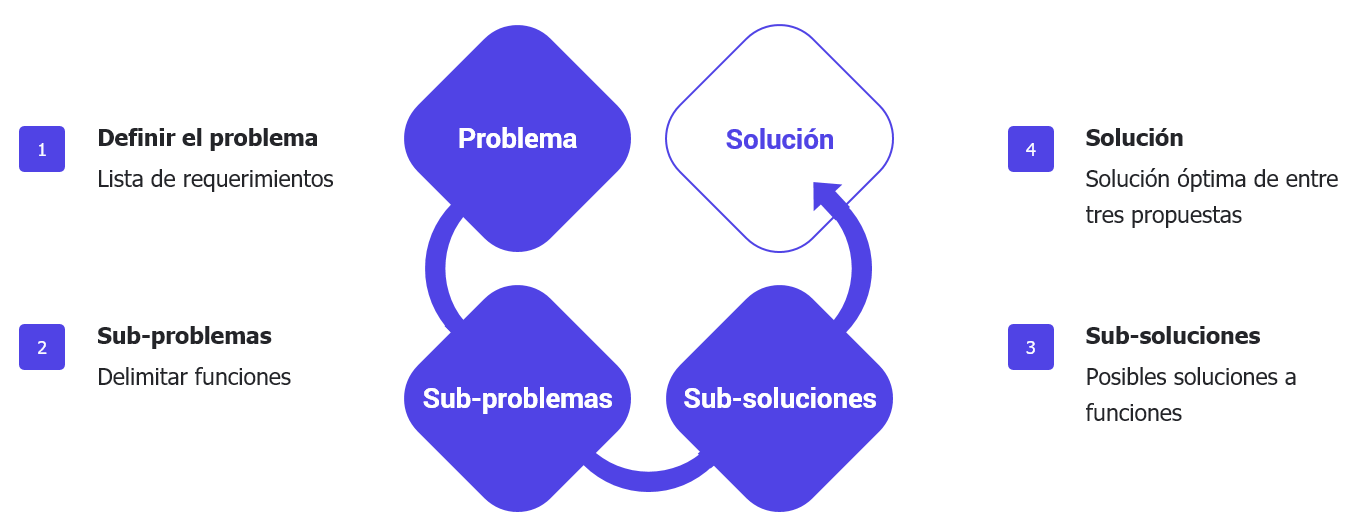
\includegraphics[width=1\textwidth]{chapter5/estado diseno subsoluciones.png}
	\caption{Estado de diseño mecatrónico: sub-soluciones}
	\begin{myflushleftportland}
		Fuente: Elaboración propia
	\end{myflushleftportland}
	\label{fig:estado diseno mecatronico etapa 3}
\end{myfigure}

Según el proceso de diseño indicado en la norma VDI 2221 que se muestra en la Figura \ref{fig:vdi2221} se parte del diseño conceptual propuesto (5) y se presenta el diseño integral (6)\footnote{\cite{Pahl2007}}, también llamado diseño de ingeniería, que abarca diferentes puntos: dimensionamiento del sistema; cálculos; selección técnica de materiales entorno a su aplicación; selección técnica de sensores; actuadores y dispositivos de control; lógica del control del sistema y su estrategia; planos mecánicos: ensamble y despiece; planos eléctricos y/o electrónicos; simulaciones de la máquina y una estimación de costos.

\begin{myfigure}[H]
	\centering
	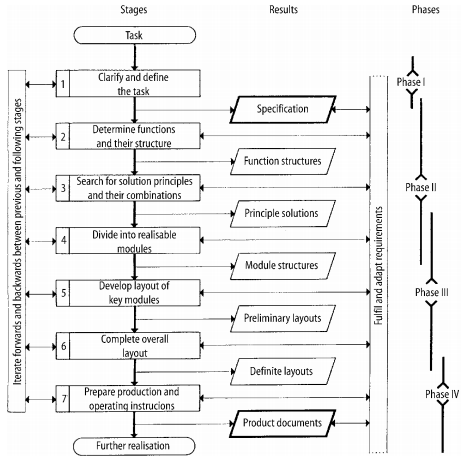
\includegraphics[width=0.75\textwidth]{chapter5/vdi2221.png}
	\caption{Fases de diseño según VDI 2221}
	\begin{myflushleftportland}
		Fuente: \cite{Pahl2007}
	\end{myflushleftportland}
	\label{fig:vdi2221}
\end{myfigure}



%% NUEVA SECCIÓN X.X.X
\subsection{Descripción del sistema integral}
\label{ssec:descripcion del sistema integral}

Dolor sit amet consectetur adipiscing elit ut aliquam purus sit. Dolor sed viverra ipsum nunc aliquet bibendum. Euismod in pellentesque massa placerat. Et malesuada fames ac turpis egestas sed tempus urna. Euismod elementum nisi quis eleifend quam adipiscing vitae proin. Ornare suspendisse sed nisi lacus sed. Mollis aliquam ut porttitor leo a diam.

%% NUEVO SUBSECCION X.X.X.X
\subsubsection{Arquitectura de hardware}

En la Figura \ref{fig:arquitectura de hardware del sistema} se muestra la propuesta de arquitectura de hardware. Esta arquitectura nos muestra las entradas de energía del sistema, su redistribución a cada componente, el control asociado a cada pieza mediante el subsistema de control y los protocolos o energía asociado a cada par de bloques. El tipo de conexión se detalla en la leyenda.

\begin{myfigure}[H]
	\centering
	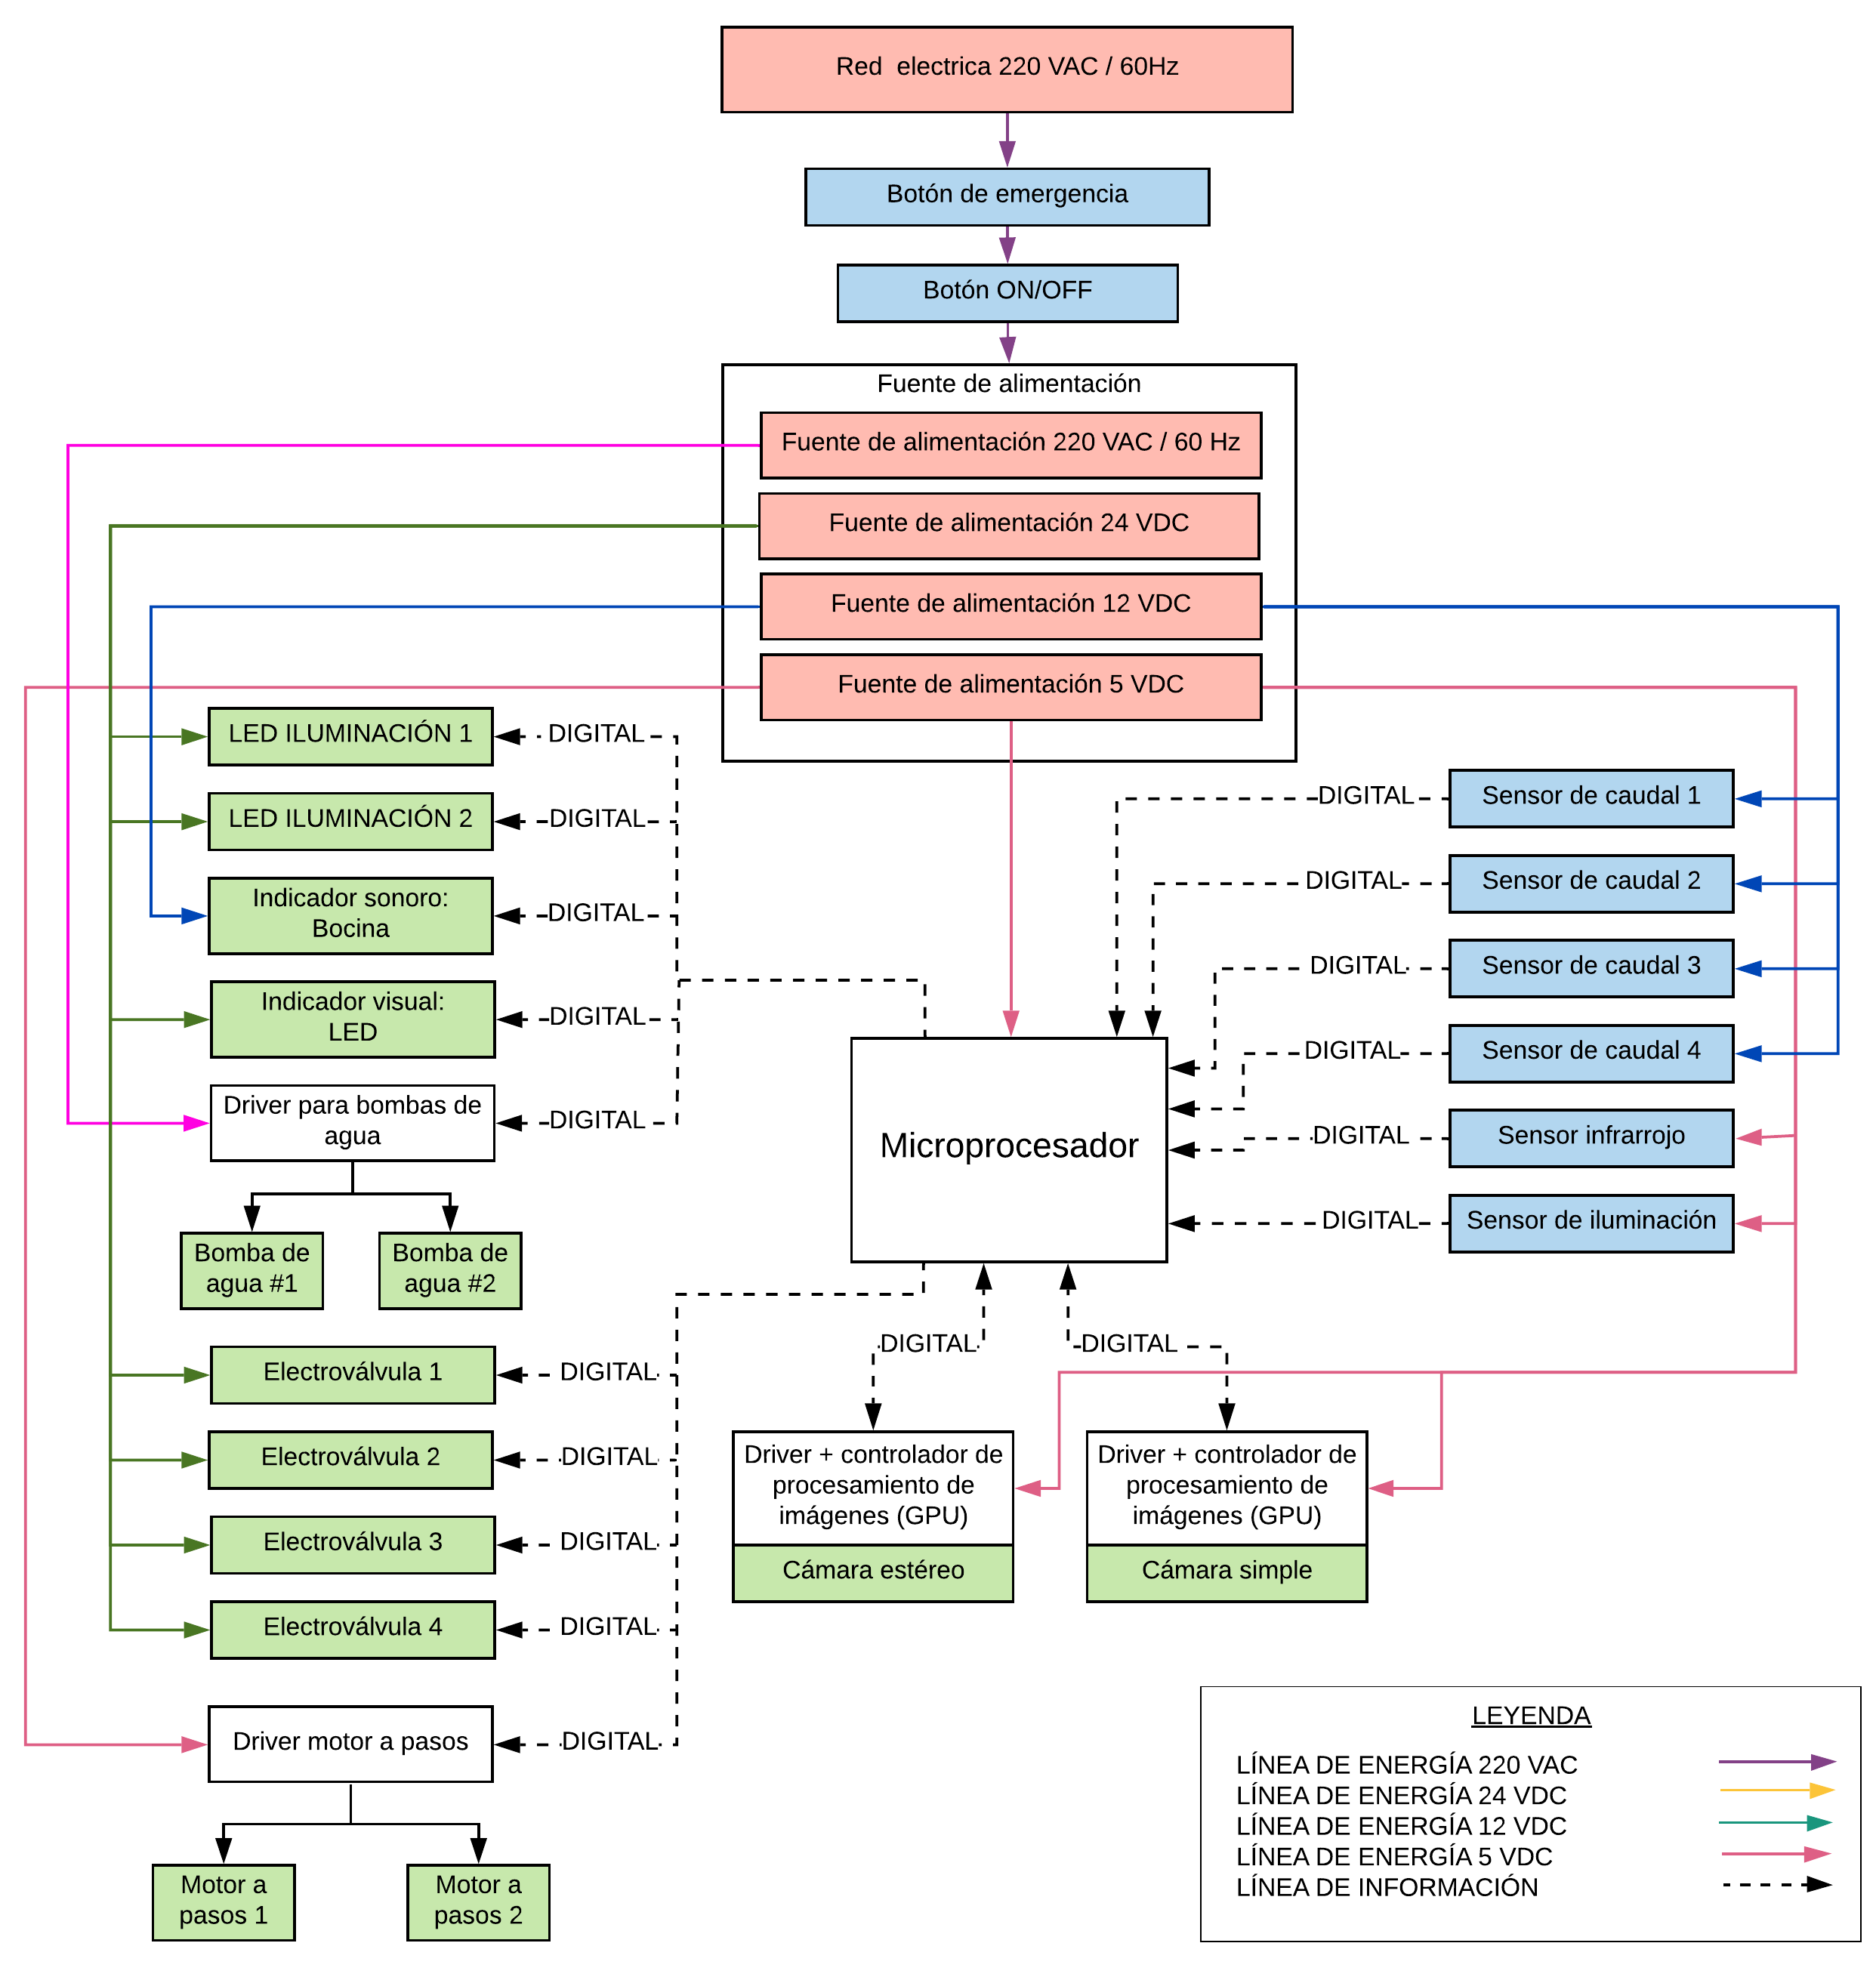
\includegraphics[width=0.75\textwidth]{chapter5/arquitectura de hardware del sistema.png}
	\caption{Arquitectura de hardware del sistema}
	\begin{myflushleftportland}
		Fuente: Elaboración propia.
	\end{myflushleftportland}
	\label{fig:arquitectura de hardware del sistema}
\end{myfigure}


Dolor sit amet consectetur adipiscing elit ut aliquam purus sit. Dolor sed viverra ipsum nunc aliquet bibendum. Euismod in pellentesque massa placerat. Et malesuada fames ac turpis egestas sed tempus urna. Euismod elementum nisi quis eleifend quam adipiscing vitae proin. Ornare suspendisse sed nisi lacus sed. Mollis aliquam ut porttitor leo a diam.

%% NUEVO SUBSECCION X.X.X.X
\subsubsection{Selección de materiales de fabricación}
\label{sssec:seleccion de materiales de fabricacion}

Cada subsistema posee mecanismos que se rigen por un material en general, esto incluye a las partes principales del subsistema. Sin embargo, no considera el material de tornillos, ajustes o dispositivos similares. Existen así mismos requisitos que se pueden generalizar para todos los subsistemas por el entorno de trabajo a la que estará sometida la máquina detallados en la \textit{"Lista de requerimientos"} \footnote{\cite{DiazVergara2020}.}. Basado en dichas demandas, cada subsistema es analizado y presentado con dos alternativas posibles de materiales. Consecuentemente, se elige un material decisivo para ser empleado bajo el sustento técnico que se explicará en los siguientes párrafos.

\begin{itemize}
	\item \textbf{Subsistema de recepción y traslado de truchas:} Cuenta con dos mecanismos; recepción de truchas y tuberías de traslado. El primero debe recepcionar a las truchas y dirigirlas al mecanismo de tuberías. El segundo debe trasladar a las truchas de un punto a otro de la máquina mediante las tuberías. En la Tabla \ref{tab:tabla comparativa de propiedades entre aluminio vs acero inoxidable} se comparan técnicamente las propiedades de dos materiales posibles.
	
	\begin{mytable}[H]
		\centering
		\caption{Tabla comparativa de propiedades entre $Aluminio$ vs $Acero Inoxidable$}
		\label{tab:tabla comparativa de propiedades entre aluminio vs acero inoxidable}
		\begin{tabular}{|l|c|c|}
			\hline
			\multicolumn{1}{|c|}{\textbf{Propiedad}} & \textbf{Aluminio} & \textbf{Acero Inoxidable} \\ \hline
			Módulo de Young ($GPa$) & 69 & 200 \\ \hline
			Esfuerzo de fatiga $Y$ ($MPa$) & 58-110 & 210-440 \\ \hline
			Resistencia a la tracción ($MPa$) & 130-410 & 580-1180 \\ \hline
			Temperatura máxima mecánica ($°C$) & 650 & 1450 \\ \hline
			Conductividad térmica ($W/m-K$) & 170 & 16 \\ \hline
			Expansión térmica (${\mu}m/m-K$) & 24 & 17 \\ \hline
			Conductividad eléctrica ($\%$) & 43 & 2.4 \\ \hline
			Densidad ($g/cm^3$) & 2.7 & 7.8 \\ \hline
		\end{tabular}
		\begin{flushleft}
			*Terminología técnica de los materiales: Aluminio 6061, Acero Inoxidable ANSI 304.\\		
			Fuente: \cite{MakeItFrom2020}.
		\end{flushleft}
	\end{mytable}

	Se elige el material Aluminio 6061 por la alta durabilidad .... ..... .........
	
	\item \textbf{Subsistema de procesamiento de imágenes:} Cuenta con dos mecanismos; tuberías y juego de espejos. El primero debe brindar a la cámara suficiente transparencia para obtener una fotografía adecuada. El segundo debe brindar a la cámara más perfiles del cuerpo que es trasladado por la tubería. En la Tabla \ref{tab:tabla comparativa de propiedades entre pmma vs pvcu} se compara técnicamente las propiedades de dos materiales posibles.
	
	\begin{mytable}[H]
		\centering
		\caption{Tabla comparativa de propiedades entre $PMMA$ vs $PVC-U$}
		\label{tab:tabla comparativa de propiedades entre pmma vs pvcu}
		\begin{tabular}{|l|c|c|}
			\hline
			\multicolumn{1}{|c|}{\textbf{Propiedad}} & \multicolumn{1}{c|}{\textbf{Acrílico}} & \textbf{PVC} \\ \hline		
			Resistencia al impacto: con muescas ($J/m$) & 74                & 360          \\ \hline
			Expansión térmica (${\mu}m/m-K$)                 & 76                & 61           \\ \hline
			Densidad ($g/cm^3$)                                   & 1.2               & 1.4          \\ \hline
			Resistencia al peso                                 & 32                & 20           \\ \hline
			Alargamiento a la rotura ($ \% $)                        & 4                 & 58           \\ \hline
		\end{tabular}
		\begin{flushleft}
			*Terminología técnica de los materiales: Cloruro de polivinilo no plastificado (rígido) (uPVC, PVC-U), Polimetilmetacrilato (Acrílico)(PMMA).\\		
			Fuente: \cite{MakeItFrom2020}.
		\end{flushleft}
	\end{mytable}

	Se elige el material Aluminio 6061 por la alta durabilidad .... ..... .........
	
	\item \textbf{Subsistema de procesamiento de suministro de energía:} Los materiales son propios de los dispositivos que serán adquiridos.
	
	\item \textbf{Subsistema de control e interacción con el usuario:} Los materiales son propios de los dispositivos que serán adquiridos.
	
	\item \textbf{Subsistema de flotación:} Cuenta con dos mecanismos; armadura y flotadores. El primero debe funcionar como esqueleto para los otros subsistemas y del mismo. El segundo debe mantener el sistema a flote.
	
\end{itemize}






\begin{mytable}[H]
	\centering
	\caption{Tabla comparativa de propiedades entre $HDPE$ vs $PVC-U$}
	\label{tab:tabla comparativa de propiedades entre hdpe vs pvcu}
	\begin{tabular}{|l|c|c|}
		\hline
		\multicolumn{1}{|c|}{\textbf{Propiedad}} & \textbf{HDPE} & \textbf{PVC-U} \\ \hline
		Densidad ($g/cm^3$) & 1.0-1.3 & 1.4 \\ \hline
		Elongación a rotura ($\%$) & 2.5-100 & 58 \\ \hline
		Resistencia al impacto ($J/m$) & 50-260 & 360 \\ \hline
		Resistencia al peso: Flexión & 19-32 & 20 \\ \hline
		Resistencia a la tracción ($MPa$) & 24-80 & 47 \\ \hline
	\end{tabular}
	\begin{flushleft}
		*Terminología técnica de los materiales: Polietileno de alta densidad (HDPE), Cloruro de polivinilo no plastificado (rígido) (uPVC, PVC-U)\\		
		Fuente: \cite{MakeItFrom2020}.
	\end{flushleft}
\end{mytable}


Los materiales de fabricación finales se muestran en la Tabla \ref{tab:materiales de fabricacion por subsistema} y fueron seleccionados por su superioridad en las propiedades que son valoradas en este proyecto. Las Tablas 

\begin{mytable}[H]
	\centering
	\caption{Materiales de fabricación por subsistema}
	\label{tab:materiales de fabricacion por subsistema}
	\begin{tabular}{|l|c|c|}
		\hline
		\multicolumn{1}{|c|}{\textbf{Subsistema}} & \multicolumn{1}{c|}{\textbf{Mecanismo}} & \textbf{Material} \\ \hline
		Recepción y traslado de truchas      & Recepción de truchas   & Acero Inoxidable            \\ \hline
		Recepción y traslado de truchas      & Tuberías de traslado   & PVC                         \\ \hline
		Procesamiento de imágenes            & Tubería                & Acrílico                    \\ \hline
		Procesamiento de imágenes            & Juego de espejos       & Cristal Acrílico    \\ \hline
		Suministro de energía                & \multicolumn{1}{c|}{-} & -                           \\ \hline
		Control e interacción con el usuario & \multicolumn{1}{c|}{-} & -                           \\ \hline
		Flotación                            & Armadura               & Aluminio o Acero Inoxidable \\ \hline
		Flotación                            & Flotadores             & HDP                         \\ \hline
	\end{tabular}
	\begin{flushleft}
	*Terminología técnica de los materiales: Cloruro de polivinilo no plastificado (rígido) (uPVC, PVC-U), Polimetilmetacrilato (Acrílico)(PMMA), Polietileno de alta densidad (HDPE), Acero Inoxidable 304, Aluminio 6061 ($AL$)\\	
	Fuente: Elaboración propia. 
	\end{flushleft}
\end{mytable}



%% NUEVA SECCIÓN X.X.X
\subsection{Subsistema de recepción y traslado de truchas}
\label{ssec:subsistema de recepcion y traslado de truchas}

Este subsistema consiste en encapsular los mecanismos físicos que están en el ciclo que sigue una trucha dentro de la máquina. 


%% NUEVO SUBSECCION X.X.X.X
\subsubsection{Diseño de tolva de recepción de truchas}

El diseño implica un análisis ....

\begin{myfigure}[H]
	\centering
	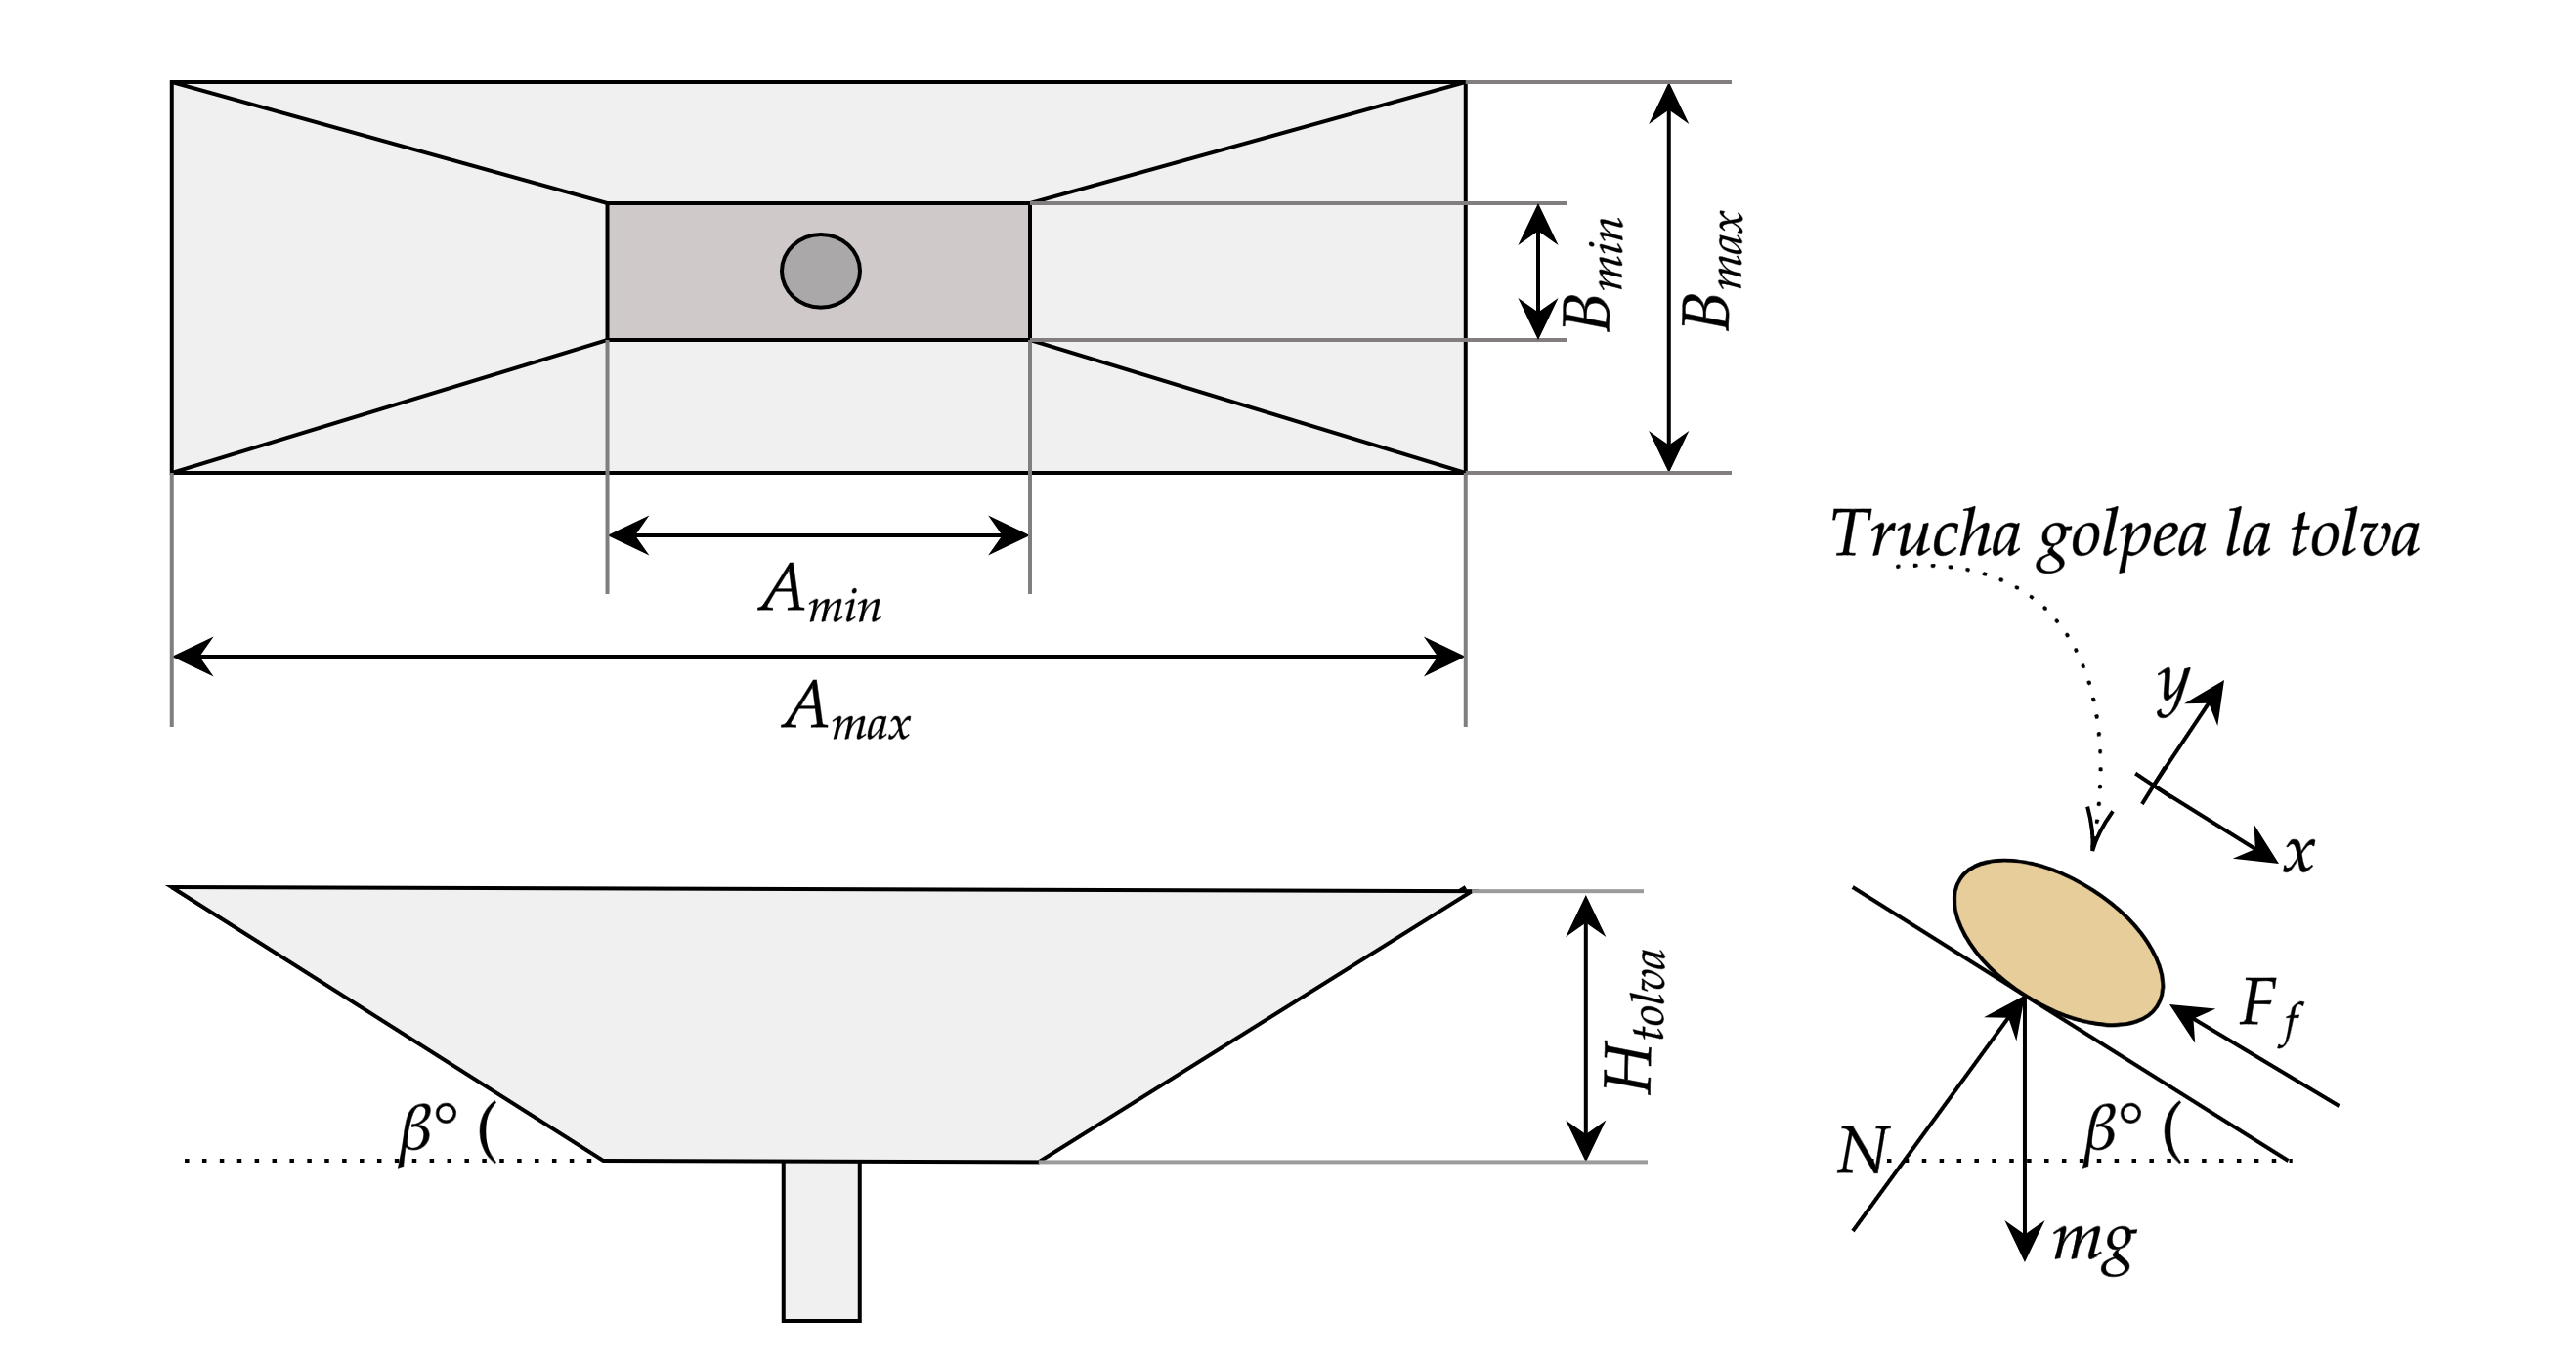
\includegraphics[width=1\textwidth]{chapter5/calculo de dimensiones y angulo de la tolva.png}
	\caption{Cálculo de dimensiones y angulo de la tolva}
	\begin{myflushleftportland}
		Fuente: Elaboración propia.
	\end{myflushleftportland}
	\label{fig:calculo de dimensiones y angulo de la tolva}
\end{myfigure}

Las leyes de Newton se muestran en la Ecuación \ref{eq:leyes de newton}

\begin{myequation}\label{eq:leyes de newton}
	\begin{split}
		F_{R}=m*a \\
		\sum_{0}^{n}F_{x,y,z}=0
	\end{split}
\end{myequation}

En la Figura \ref{fig:calculo de dimensiones y angulo de la tolva} se muestra el diagrama de cuerpo libre del cual se extrae la fuerza de fricción ($F_{f}$) y la fuerza normal ($N$) que se muestran en la Ecuación \ref{eq:calculo de angulo de la tolva}

\begin{myequation}\label{eq:calculo de angulo de la tolva}
	\begin{split}
		F_{f}=\mu*N  \\
		\sum_{}^{}F_{y}=N-mg*cos(\beta)=0
	\end{split}
\end{myequation}



\begin{myequation}\label{eq:calculo de angulo de la tolva2}
	\begin{split}
		mg*sin(\beta)-F_{f}&=m*\ddot{x} \\
		mg*sin(\beta)-\mu_{k}*mg*cos(\beta)&=m*\ddot{x} \\
		g*sin(\beta)-g*\mu_{k}*cos(\beta)&=\ddot{x}
	\end{split}
\end{myequation}

Para disminuir el impacto de la trucha sobre la tolva o sobre las tuberías interiores se debe disminuir la aceleración de la trucha al ser depositada en la tolva. La Figura \ref{fig:grafico angulo de tolva vs aceleracion} muestra la ecuación que relaciona la aceleración con el ángulo de elevación de la pared de la tolva. Consecuentemente, se escoge un ángulo ($\beta=30°$) para tener una aceleración aproximadamente nula ($\ddot{x}\approx0$). Se considera $\mu_{k}=0.57$ para el material escogido en la sección \ref{sssec:seleccion de materiales de fabricacion}.

% Material escogido Acero inoxidable

\begin{myfigure}[H]
	\centering
	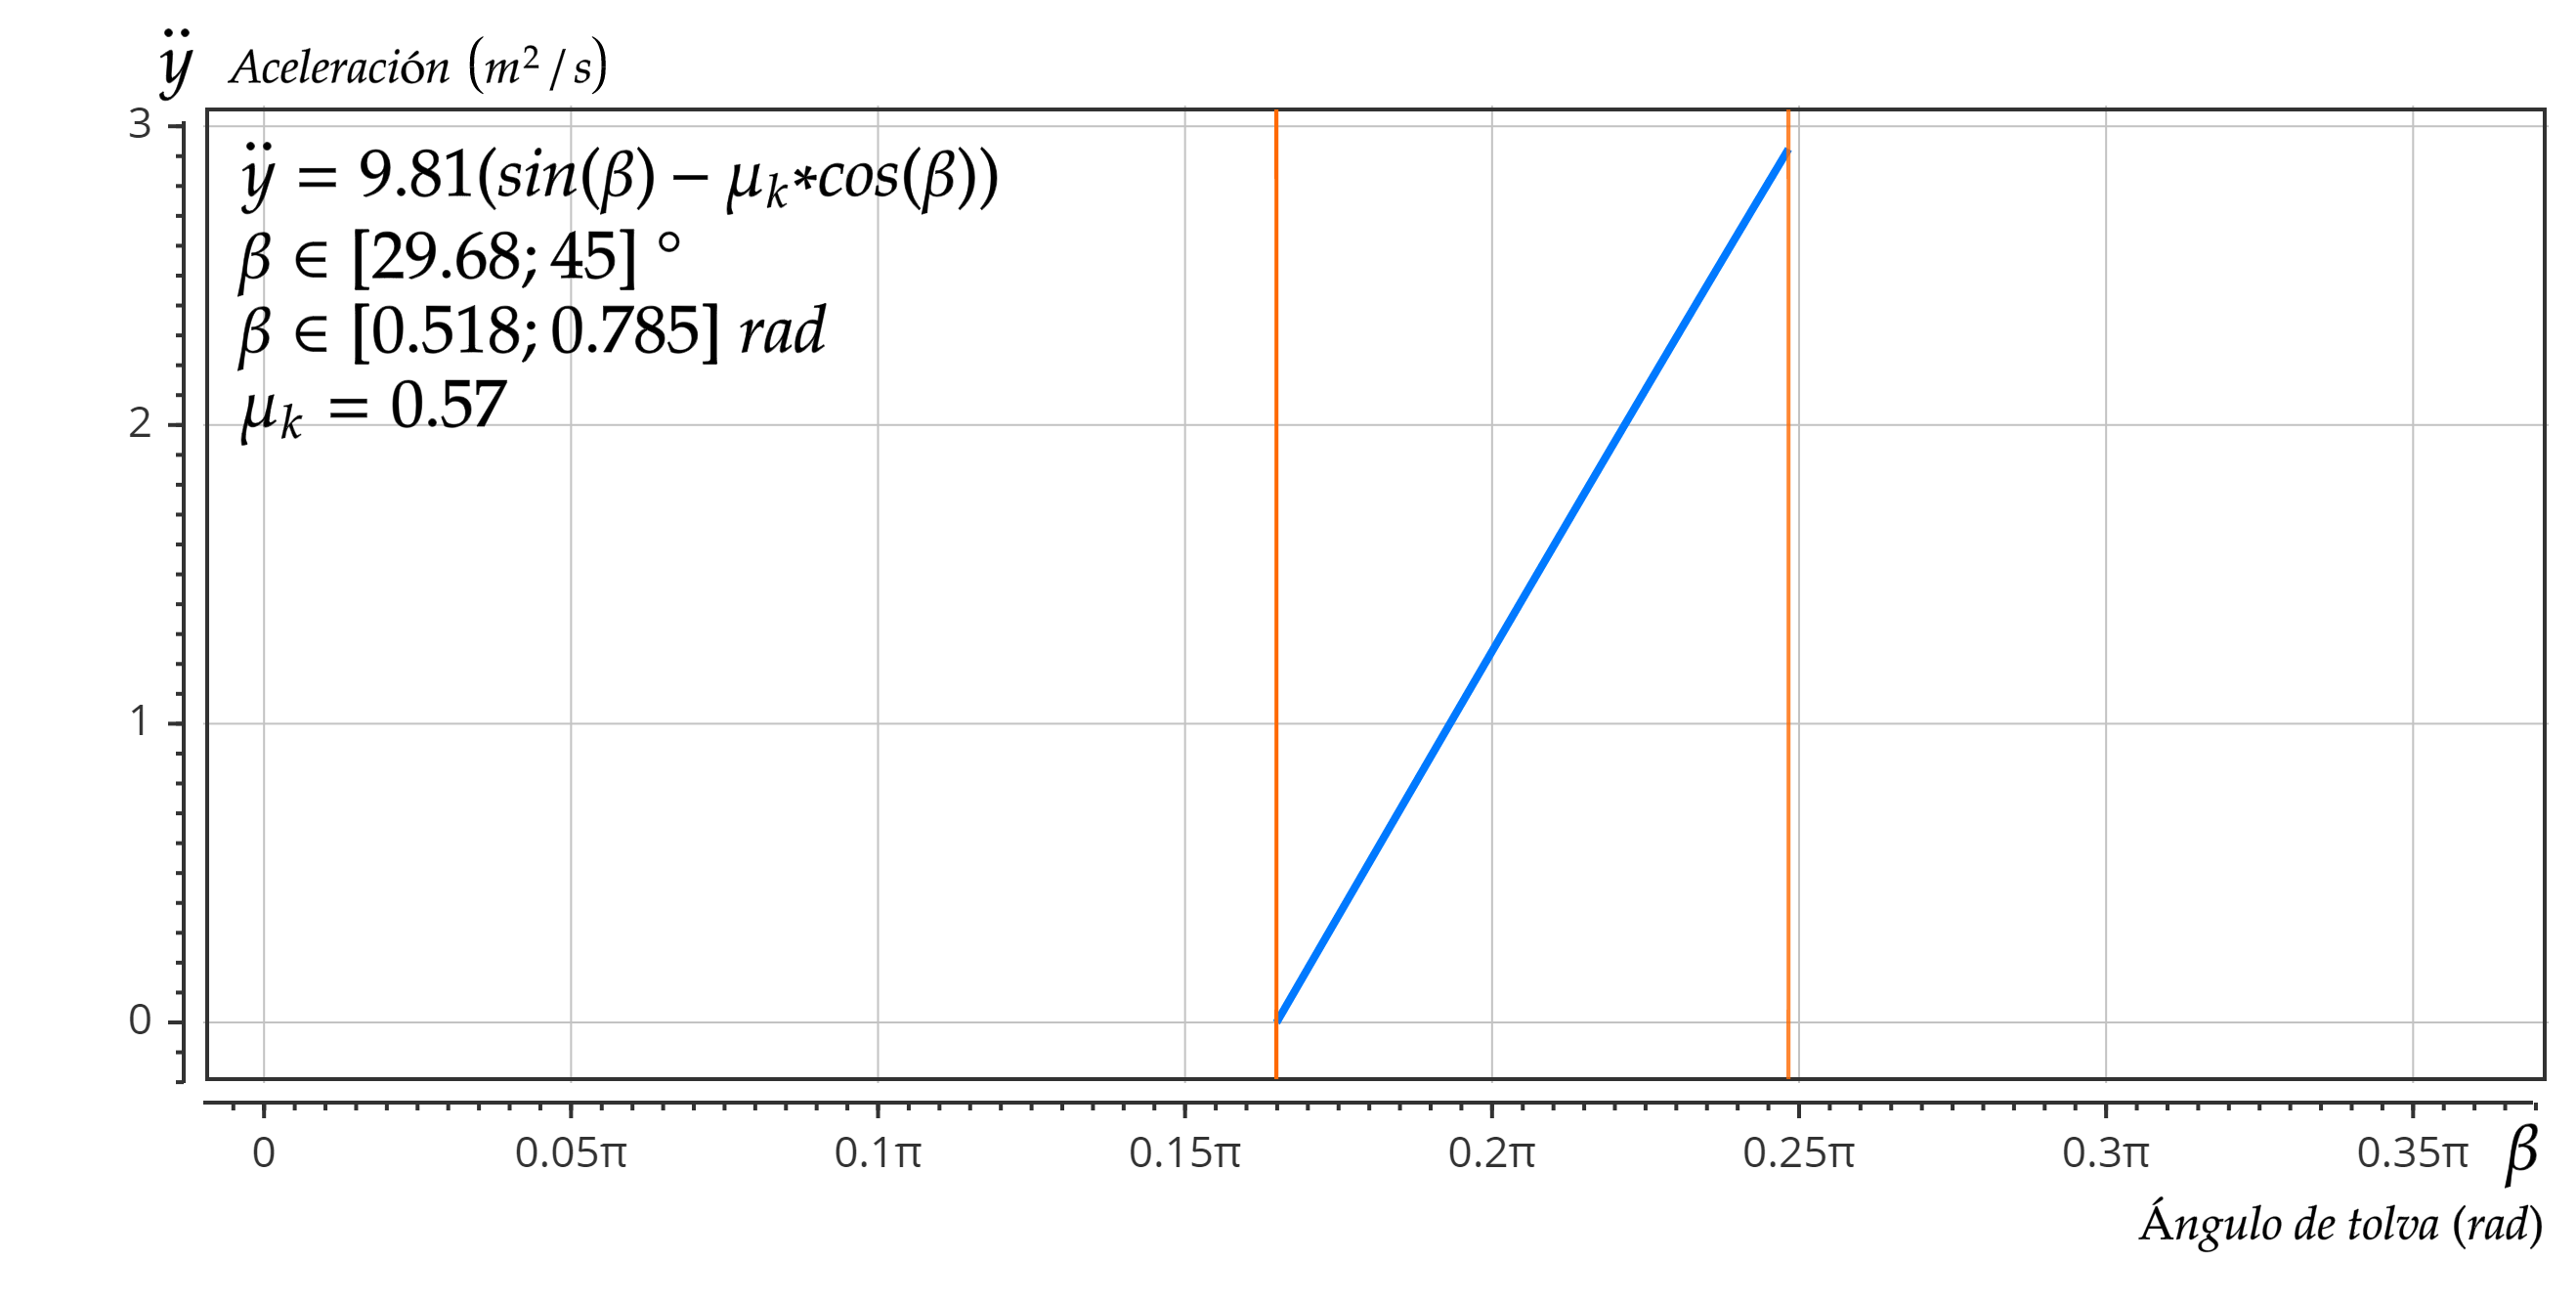
\includegraphics[width=1\textwidth]{chapter5/grafico angulo de tolva vs aceleracion.png}
	\caption{Ángulo de tolva vs aceleración en la trucha}
	\begin{myflushleftportland}
		Fuente: Elaboración propia.
	\end{myflushleftportland}
	\label{fig:grafico angulo de tolva vs aceleracion}
\end{myfigure}

%% NUEVO SUBSECCION X.X.X.X
\subsubsection{Selección de reja accionada por motor}

Esta compuerta puede ser reemplazada por una tapa para la tolva de recepción de truchas. En el presente trabajo se decide optar por eliminar este componente.

%% NUEVO SUBSECCION X.X.X.X
\subsubsection{Selección de bomba sumergible}

Lorem ipsum dolor sit amet, consectetur adipiscing elit, sed do eiusmod tempor incididunt ut labore et dolore magna aliqua. Lacus sed turpis tincidunt id aliquet. Nunc aliquet bibendum enim facilisis gravida neque convallis a. Ut tellus elementum sagittis vitae et leo duis ut diam. Dolor sit amet consectetur adipiscing elit ut aliquam purus sit. Dolor sed viverra ipsum nunc aliquet bibendum. Euismod in pellentesque massa placerat. Et malesuada fames ac turpis egestas sed tempus urna. Euismod elementum nisi quis eleifend quam adipiscing vitae proin. Ornare suspendisse sed nisi lacus sed. Mollis aliquam ut porttitor leo a diam. Varius morbi enim nunc faucibus. Sit amet purus gravida quis blandit turpis cursus in hac.

%% NUEVO SUBSECCION X.X.X.X


%% NUEVO SUBSECCION X.X.X.X




%% NUEVO SUBSECCION X.X.X.X
\subsubsection{Diseño de subsistema de distribución de truchas}

Luego del proceso de procesamiento de imágenes el sistema mediante el algoritmo de clasificación dirige a la trucha en tránsito a la salida correspondiente en el mecanismo de distribución de truchas. Dicho mecanismo recibe a la trucha y debe redirigir mediante un juego de compuertas a tres salidas que a su vez se impulsan mediante un caudal a sus respectivas jaulas flotantes.

\begin{itemize}
	
	\item \textbf{Cálculo de fuerza y velocidad de compuertas}
	La fuerza necesaria es simplemente el giro de la compuerta que está unida a un eje y a su vez al mecanismo de engranajes con el servomotor.
	
	\begin{myfigure}[H]
		\centering
		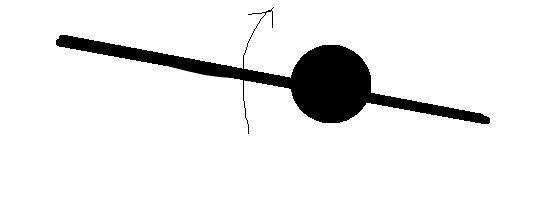
\includegraphics[width=1\textwidth]{chapter5/compuerta.png}
		\caption{Compuerta}
		\begin{myflushleftportland}
			Fuente: Elaboración propia.
		\end{myflushleftportland}
		\label{fig:compuerta}
	\end{myfigure}
	
	La velocidad de compuertas debe ir acorde a la distancia entre una trucha y la siguiente a esta. 
	
	\begin{myfigure}[H]
		\centering
		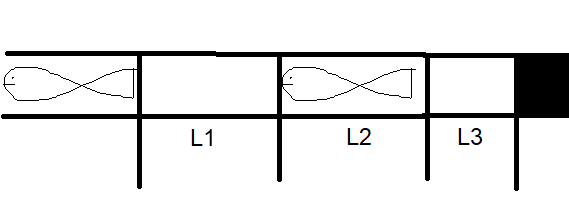
\includegraphics[width=1\textwidth]{chapter5/velocidad de compuerta.png}
		\caption{Velocidad de compuerta}
		\begin{myflushleftportland}
			Fuente: Elaboración propia.
		\end{myflushleftportland}
		\label{fig:velocidad de compuerta}
	\end{myfigure}

	Ut tellus elementum sagittis vitae et leo duis ut diam. Dolor sit amet consectetur adipiscing elit ut aliquam purus sit. 
	
	\begin{myequation}\label{eq:calculo de tiempo necesario}
		\begin{split}
			L_1+L_2+L_3 &= t * v
		\end{split}		
	\end{myequation}

	Ut tellus elementum sagittis vitae et leo duis ut diam. Dolor sit amet consectetur adipiscing elit ut aliquam purus sit. 

	
	\item \textbf{Selección de servomotores}
		
	Calcular: \\
	- Torque necesario \\
	- Condiciones de uso (estará en agua) \\
	- Tiempo de uso \\
	
	La selección de los servomotores depende del propósito en la función que se encuentre................
	
	\begin{itemize}
		
		%\item \textbf{Servomotor 1: } Este servomotor apoya en la función de \textit{accionar recepción de truchas}. 
		
		\item \textbf{Servomotor de compuerta}
		
		Este servomotor acciona la compuerta presentada en la Figura \ref{fig:compuerta}. El torque necesario del eje es $T_{max}=X (M*mm)$  y gracias al mecanismo de engranajes puede reducirse a $T_{max_2}=Y (M*mm)$ En la Tabla XXX se muestra una comparación técnica entre tres servomotores que cumplen los requerimientos técnicos y conceptuales.
		
	\end{itemize}


	\item \textbf{Diseño de mecanismo servomotor-compuerta} 
	
	Ut tellus elementum sagittis vitae et leo duis ut diam. Dolor sit amet consectetur adipiscing elit ut aliquam purus sit. 
	
	\begin{myfigure}[H]
		\centering
		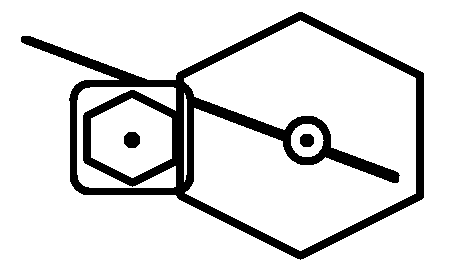
\includegraphics[width=1\textwidth]{chapter5/mecanismo servomotor-compuerta.png}
		\caption{Mecanismo servomotor-compuerta}
		\begin{myflushleftportland}
			Fuente: Elaboración propia.
		\end{myflushleftportland}
		\label{fig:mecanismo servomotor-compuerta}
	\end{myfigure}
	
	Ut tellus elementum sagittis vitae et leo duis ut diam. Dolor sit amet consectetur adipiscing elit ut aliquam purus sit. 
	
	\begin{myfigure}[H]
		\centering
		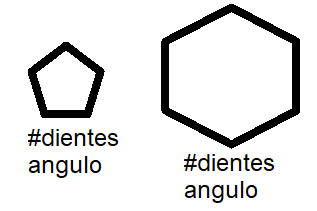
\includegraphics[width=1\textwidth]{chapter5/mecanismo de compuertas engranajes.png}
		\caption{Engranajes del mecanismo de compuertas}
		\begin{myflushleftportland}
			Fuente: Elaboración propia.
		\end{myflushleftportland}
		\label{fig:mecanismo de compuertas engranajes}
	\end{myfigure}
	
	Ut tellus elementum sagittis vitae et leo duis ut diam. Dolor sit amet consectetur adipiscing elit ut aliquam purus sit. 
	
	
	\item \textbf{Diseño de juego de compuertas programables}
	
	Descripción.

\end{itemize}



%% NUEVO SUBSECCION X.X.X.X
\subsubsection{Diseño de subsistema de tuberías}

Las tuberías del sistema tienen como propósito abastecer de un caudal a la máquina.

Lacus sed turpis tincidunt id aliquet. Nunc aliquet bibendum enim facilisis gravida neque convallis a. Ut tellus elementum sagittis vitae et leo duis ut diam. Dolor sit amet consectetur adipiscing elit ut aliquam purus sit. 

\begin{itemize}
	
	\item \textbf{Diseño de tuberías}
	
	Nunc aliquet bibendum enim facilisis gravida neque convallis a. Ut tellus elementum sagittis vitae et leo duis ut diam. Dolor sit amet consectetur adipiscing elit ut aliquam purus sit. Dolor sed viverra ipsum nunc aliquet bibendum. Euismod in pellentesque massa placerat. Et malesuada fames ac turpis egestas sed tempus urna. Euismod elementum nisi quis eleifend quam adipiscing vitae proin. Ornare suspendisse sed nisi lacus sed.
	
	\begin{myfigure}[H]
		\centering
		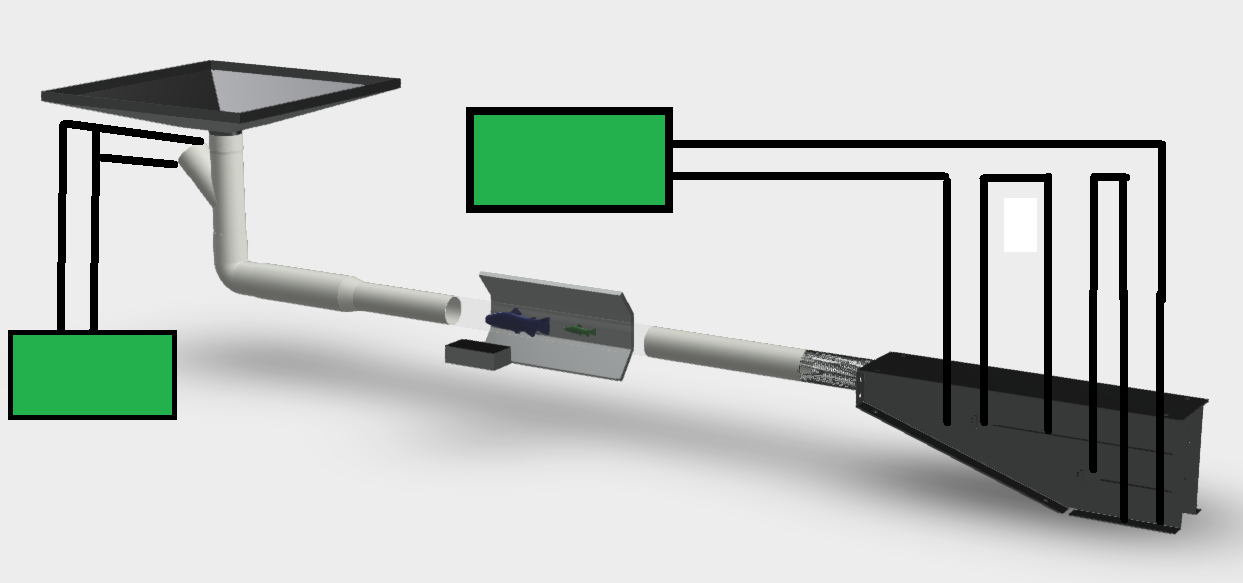
\includegraphics[width=1\textwidth]{chapter5/concepto optimo tuberias.png}
		\caption{Diseño de tuberías para el concepto óptimo}
		\begin{myflushleftportland}
			Fuente: Elaboración propia.
		\end{myflushleftportland}
		\label{fig:concepto optimo tuberias}
	\end{myfigure}

	Diseño de filtro único incluido
	
	Nunc aliquet bibendum enim facilisis gravida neque convallis a. Ut tellus elementum sagittis vitae et leo duis ut diam. Dolor sit amet consectetur adipiscing elit ut aliquam purus sit. Dolor sed viverra ipsum nunc aliquet bibendum. Euismod in pellentesque massa placerat. Et malesuada fames ac turpis egestas sed tempus urna. Euismod elementum nisi quis eleifend quam adipiscing vitae proin. Ornare suspendisse sed nisi lacus sed.	
	
	\begin{myfigure}[H]
		\centering
		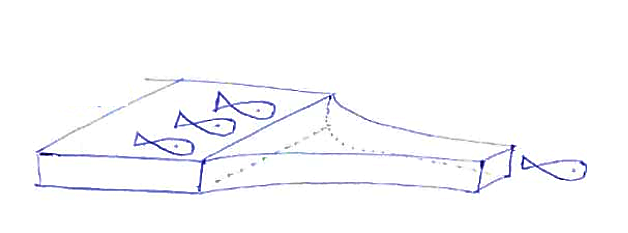
\includegraphics[width=0.25\textwidth]{chapter5/filtro unico.png}
		\caption{Filtro único}
		\begin{myflushleftportland}
			Fuente: Elaboración propia.
		\end{myflushleftportland}
		\label{fig:filtro unico}
	\end{myfigure}

	\item \textbf{Selección de caudales apropiados} 

	En la Sección \ref{sssec:seleccion de microcontrolador} se calculó la velocidad máxima, aproximada, de nado de las truchas arcoíris: $16 (cm/s)$. La Ecuación \ref{eq:calculo de caudal maximo} toma el valor de \textit{$v_{max}=16 (cm/s)$}  y el 
	
	\begin{myequation}\label{eq:calculo de caudal maximo}
		\begin{split}
			Q_{max} & = v_{max}*A \\
			Q_{max} & = 16*\frac{\pi}{4}*(r_{int})^2 \\
			Q_{max} & = 16*\frac{\pi}{4}*(9.1)^2 \\
			Q_{max} & = 1040.62 \\
		\end{split}		
	\end{myequation}
	Donde: $Q_{max} (cm^3/s)$ es el caudal máximo, $v_{max} (cm/s)$ es la velocidad máxima del agua, $r_{int} (cm)$
	
	Lorem ipsum dolor sit amet, consectetur adipiscing elit, sed do eiusmod tempor incididunt ut labore et dolore magna aliqua. Lacus sed turpis tincidunt id aliquet. Nunc aliquet bibendum enim facilisis gravida neque convallis a. Ut tellus elementum sagittis vitae et leo duis ut diam. Dolor sit amet consectetur adipiscing elit ut aliquam purus sit.	

	
	\item \textbf{Selección de las electroválvulas}
	
	Los valores límites que se tendrían que controlar mediante las electroválvulas pertenecen al rango $[0;12345] (m^3/s)$. En la Tabla XXX se muestran algunas marcas que cumplen con estos requerimientos.
	
	
	\begin{myfigure}[H]
		\centering
		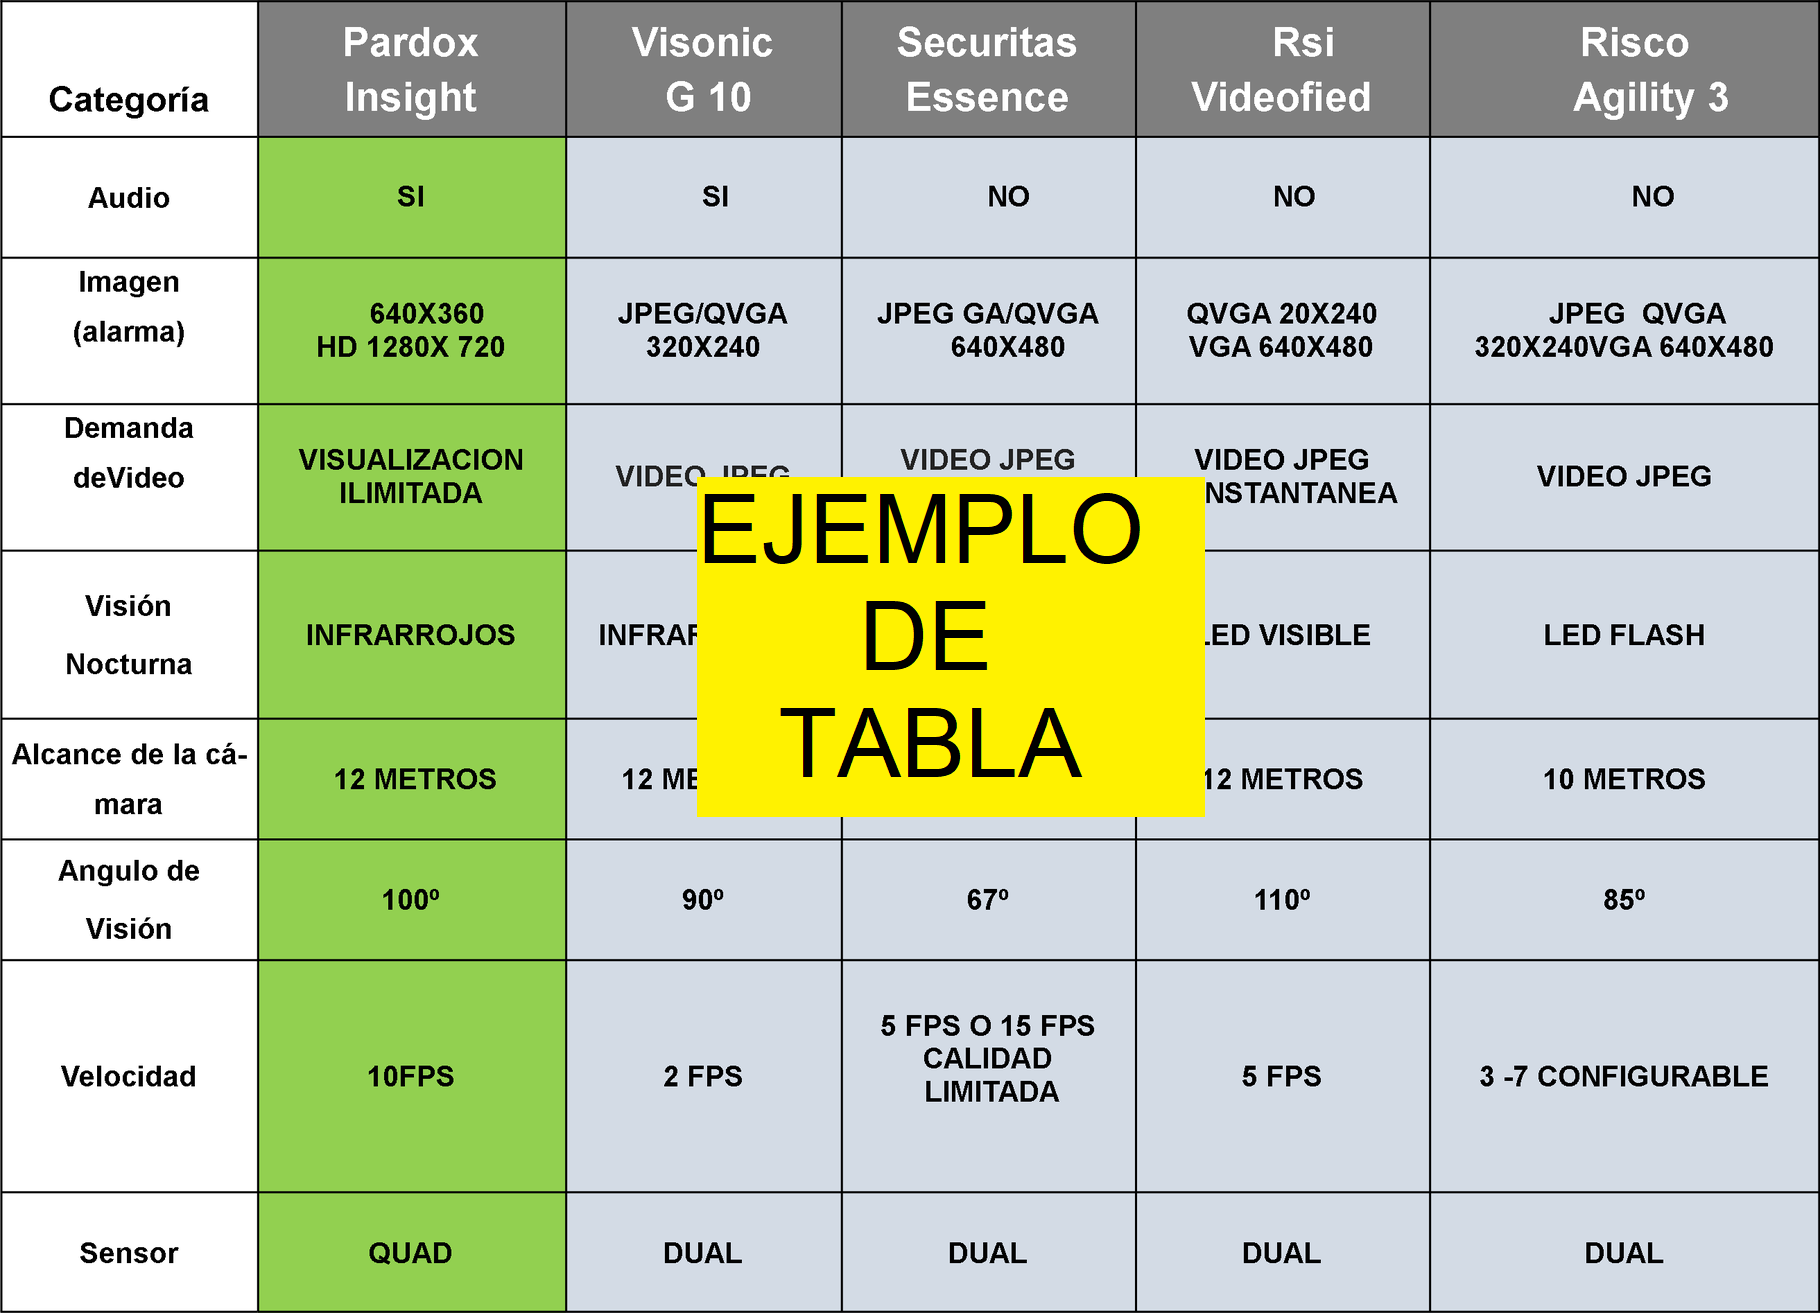
\includegraphics[width=0.85\textwidth]{chapter5/ejemplo de tabla.png}
		\caption{Ejemplo de tabla}
		\begin{myflushleftportland}
			Fuente: Elaboración propia.
		\end{myflushleftportland}
		\label{fig:ejemplo de tabla}
	\end{myfigure}
	
	Las características técnicas que se muestran en la Tabla XXX muestran que ................................
	
	Et malesuada fames ac turpis egestas sed tempus urna. Euismod elementum nisi quis eleifend quam adipiscing vitae proin. Ornare suspendisse sed nisi lacus sed. Mollis aliquam ut porttitor leo a diam. Varius morbi enim nunc faucibus. Sit amet purus gravida quis blandit turpis cursus in hac.
	
	\item \textbf{Control de los caudales de agua}
	
	Los caudales que generan las bombas de agua sirven para impulsar a las truchas por el interior de la máquina. 
	
	
	\begin{myfigure}[H]
		\centering
		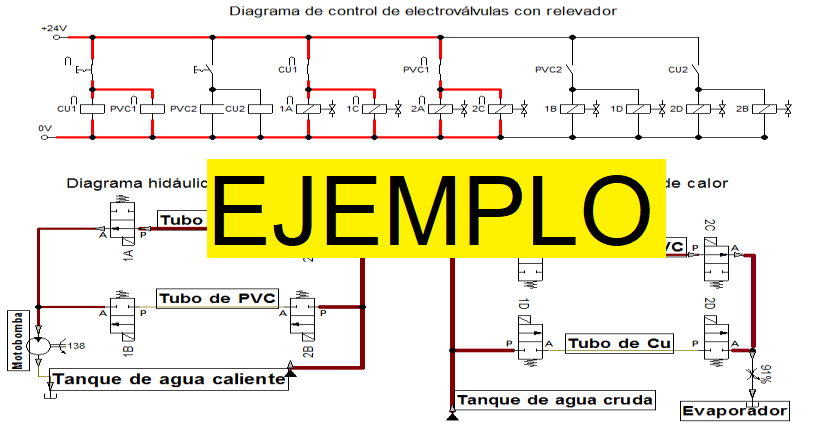
\includegraphics[width=1\textwidth]{chapter5/diagrama de control de electrovalvulas.png}
		\caption{Diagrama de control de electrovalvulas}
		\begin{myflushleftportland}
			Fuente: Elaboración propia.
		\end{myflushleftportland}
		\label{fig:diagrama de control de electrovalvulas}
	\end{myfigure}

	Lacus sed turpis tincidunt id aliquet. Nunc aliquet bibendum enim facilisis gravida neque convallis a. Ut tellus elementum sagittis vitae et leo duis ut diam. Dolor sit amet consectetur adipiscing elit ut aliquam purus sit. 
	
	\begin{myfigure}[H]
		\centering
		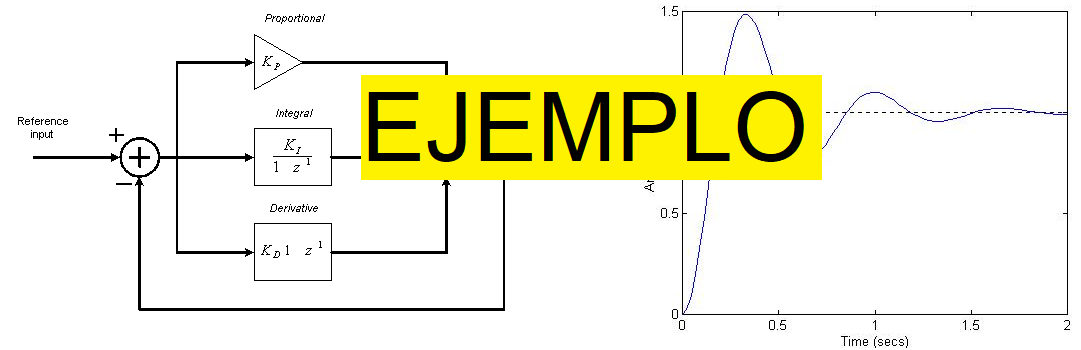
\includegraphics[width=1\textwidth]{chapter5/control electrovalvulas pid.png}
		\caption{Control PID de una electrovalvula}
		\begin{myflushleftportland}
			Fuente: Elaboración propia.
		\end{myflushleftportland}
		\label{fig:control electrovalvulas pid}
	\end{myfigure}
	
	Lacus sed turpis tincidunt id aliquet. Nunc aliquet bibendum enim facilisis gravida neque convallis a. Ut tellus elementum sagittis vitae et leo duis ut diam. Dolor sit amet consectetur adipiscing elit ut aliquam purus sit. 


\end{itemize}

%% NUEVA SECCIÓN X.X.X
\subsection{Subsistema de procesamiento de imágenes}
\label{ssec:subsistema de procesamiento de imágenes}

Este subsistema consiste obtener una serie de imágenes de una trucha en tránsito e indicar al sistema a dónde debería dirigirse una trucha determinada. El subsistema debe clasificar y contar truchas, con dicha finalidad necesita de la selección de una cámara y generar el ambiente adecuado para obtener las imágenes. Explicado los objetivos del subsistema, en las siguientes líneas se detalla: la selección del sensor infrarrojo, la selección de cámara estéreo, la selección de iluminación adecuada y la selección de algoritmos.

%% NUEVO SUBSECCION X.X.X.X
\subsubsection{Selección del sensor infrarrojo}

El sensor infrarrojo tiene como objetivo activar el algoritmo de detección y conteo de truchas por un determinado periodo de tiempo con la finalidad de evitar un sobre uso de los recursos computacionales. El sensor infrarrojo está unos centímetros antes de la parte que la cámara captura y su posición es como se muestra en las Figura \ref{fig:posicion sensor infrarrojo}.

\begin{myfigure}[H]
	\centering
	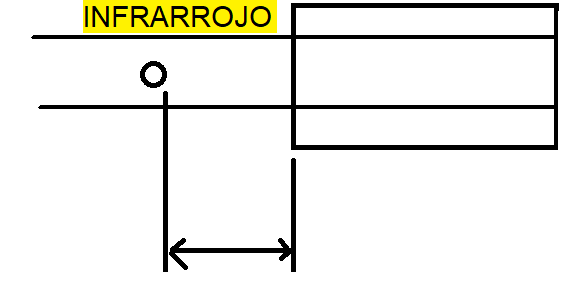
\includegraphics[width=0.5\textwidth]{chapter5/posicion sensor infrarrojo.png}
	\caption{Posicionamiento del sensor infrarrojo}
	\begin{myflushleftportland}
		Fuente: Elaboración propia.
	\end{myflushleftportland}
	\label{fig:posicion sensor infrarrojo}
\end{myfigure}

Entonces, el sensor infrarrojo debe tener un tiempo de respuesta ........ ........ Las comparaciones técnicas de los dispositivos comerciales que cumplen este requerimiento se muestran en la Tabla XXX.

\begin{myfigure}[H]
	\centering
	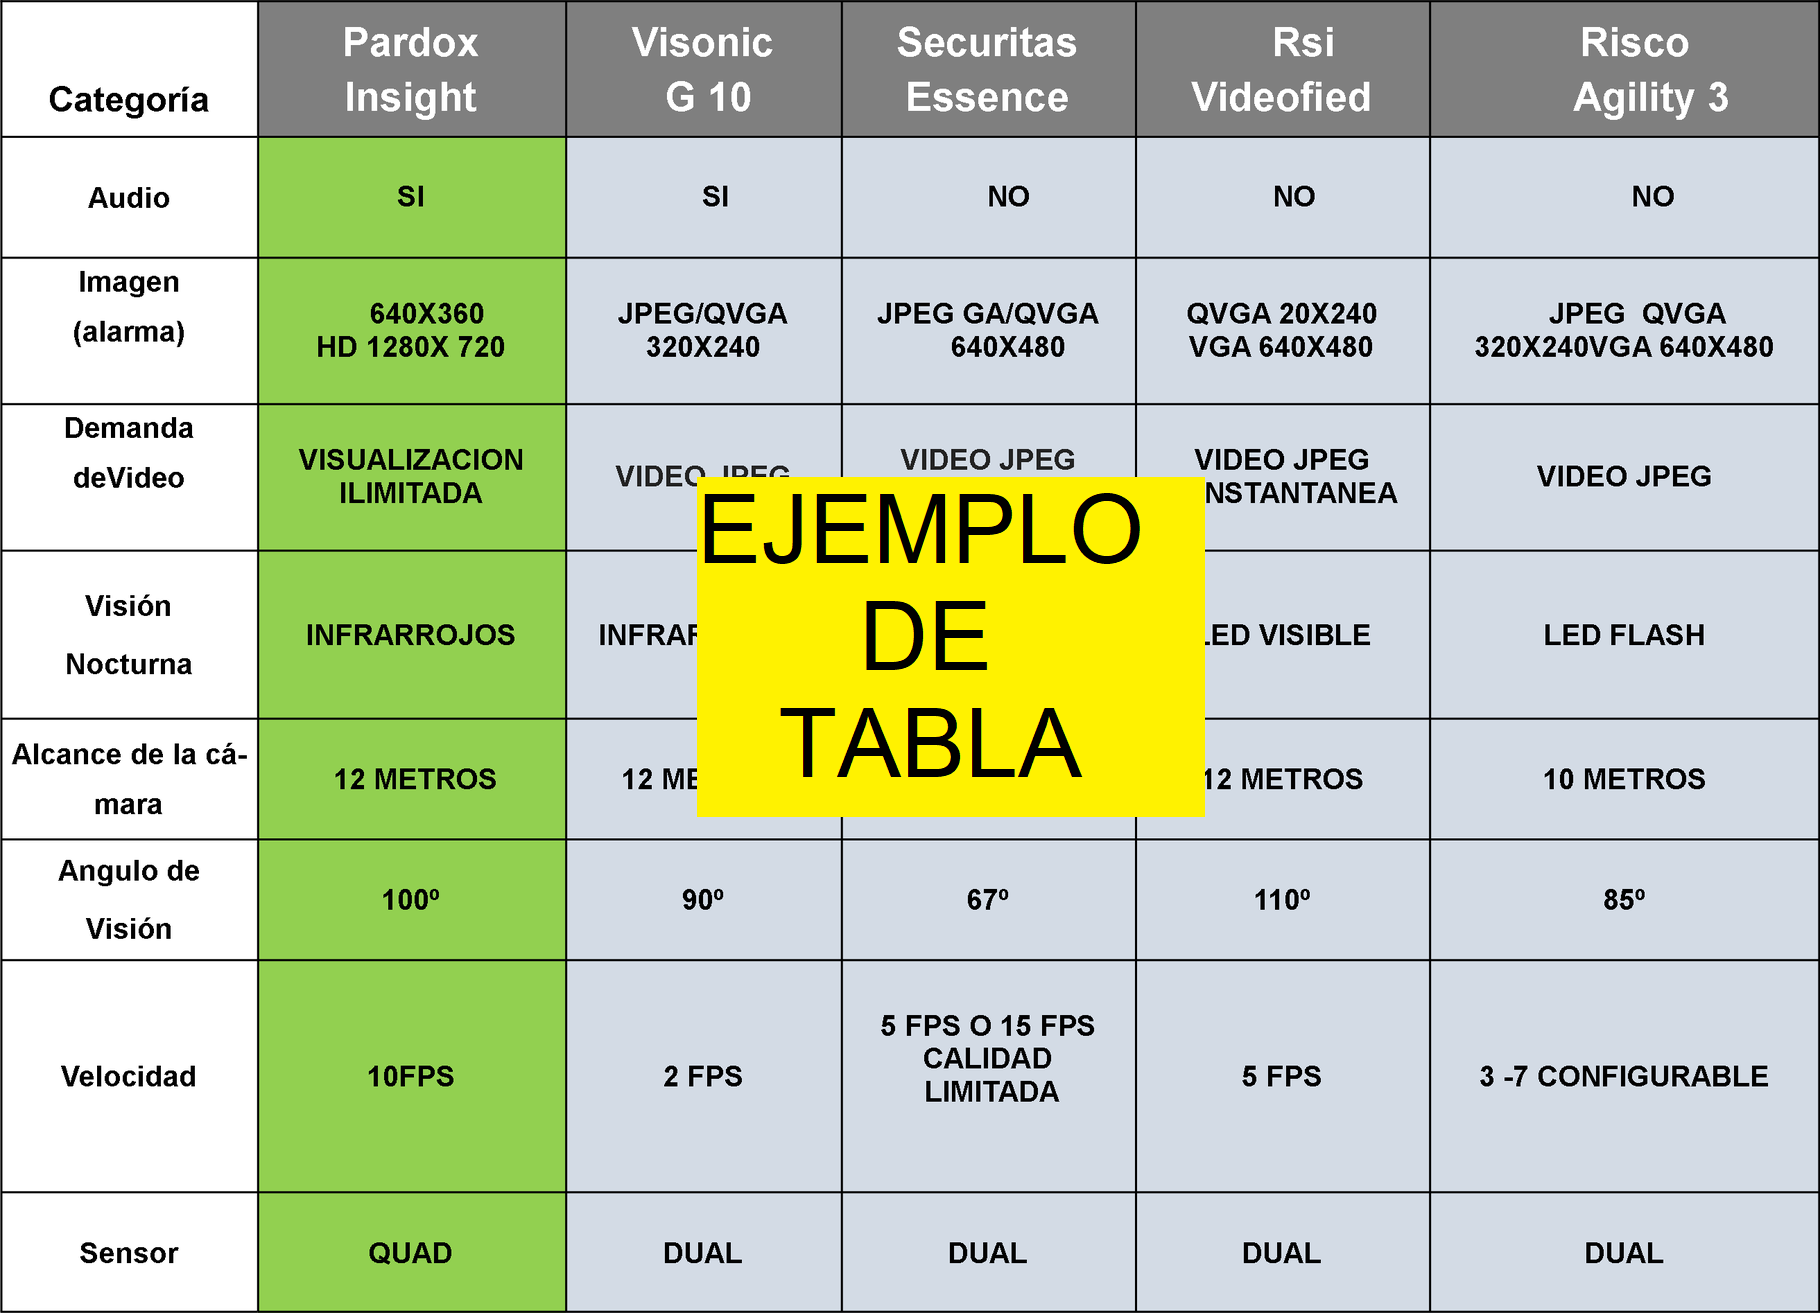
\includegraphics[width=0.85\textwidth]{chapter5/ejemplo de tabla.png}
	\caption{Ejemplo de tabla}
	\begin{myflushleftportland}
		Fuente: Elaboración propia.
	\end{myflushleftportland}
	\label{fig:ejemplo de tabla}
\end{myfigure}

%% NUEVO SUBSECCION X.X.X.X
\subsubsection{Selección de cámaras} 

Euismod in pellentesque massa placerat. Et malesuada fames ac turpis egestas sed tempus urna. Euismod elementum nisi quis eleifend quam adipiscing vitae proin.Euismod in pellentesque massa placerat. Et malesuada fames ac turpis egestas sed tempus urna. Euismod elementum nisi quis eleifend quam adipiscing vitae proin.

\begin{itemize}
	\item \textbf{Cámara estéreo}
	
	El objetivo de la cámara estéreo es la de obtener fotos por determinado periodo de tiempo designado por los algoritmos de procesamiento de imágenes. Con el fin de cumplir el objetivo mencionado deben cumplirse requerimientos: fotografiar a la trucha con un enfoque aceptable que permita distinguir a la trucha adecuadamente.
	
	Cómo mide la cámara estéreo 
	
	El error realizado en pruebas con vehículos autónomos brindado en \cite{Zaarane2020} se muestra en la Figura \ref{fig:medicion de distancia con distintas distancias}
	
	\begin{myfigure}[H]
		\centering
		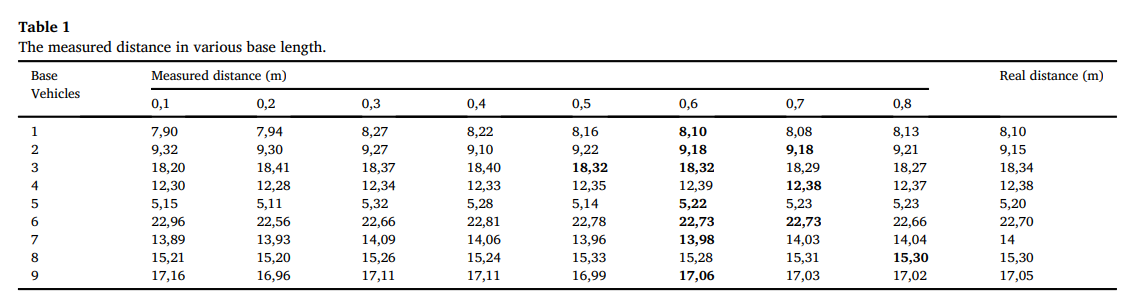
\includegraphics[width=1\textwidth]{chapter5/medicion de distancia con distintas distancias.png}
		\caption{Pruebas de medición con distintas distancias al objeto.}
		\begin{myflushleftportland}
			Fuente: \cite{Zaarane2020}
		\end{myflushleftportland}
		\label{fig:medicion de distancia con distintas distancias}
	\end{myfigure}
	
	
	\begin{myfigure}[H]
		\centering
		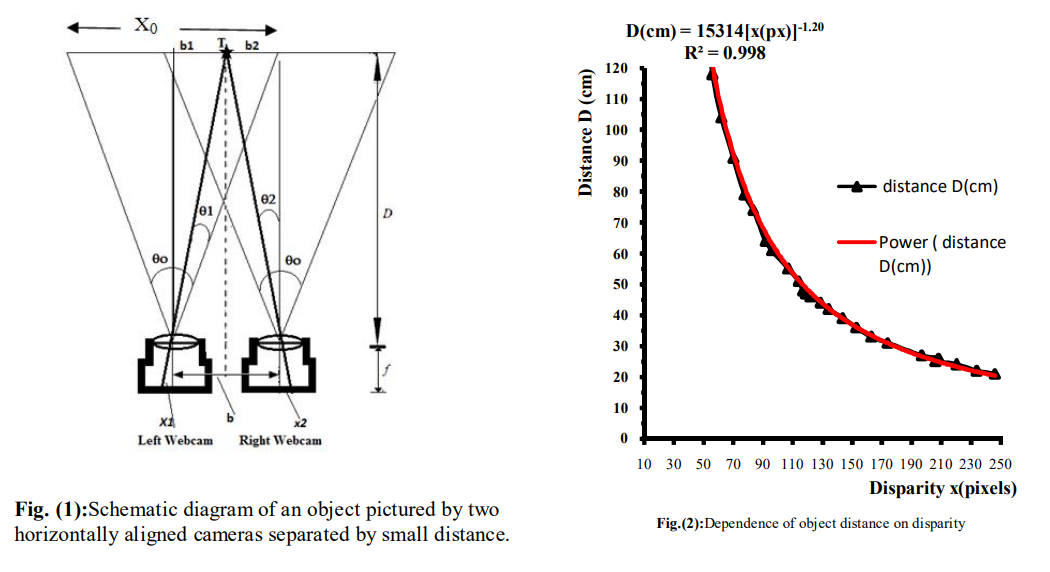
\includegraphics[width=1\textwidth]{chapter5/diagrama esquematico camara estereo y dependencia de la distancia del objeto.png}
		\caption[Diagrama esquemático y dependencia de la distancia del objeto seguido por una cámara estéreo.]{(Izq.) Diagrama esquemático de un objeto representado por dos cámaras alineadas horizontalmente separadas por una pequeña distancia. (Der.) Dependencia de la distancia del objeto en la disparidad.}
		\begin{myflushleftportland}
			Fuente: \cite{Mahammed2013}
		\end{myflushleftportland}
		\label{fig:diagrama esquematico camara estereo y dependencia de la distancia del objeto}
	\end{myfigure}
	
	
	Tener en cuenta: \\
	- Tamaño de píxeles requerido \\
	- Cantidad de frames (80 fps con 3-4L/s) (Falta calcular con lo que hemos calculado 16 cm/s) \\ 
	- La inclinación hace que el pez no tenga velocidad hacia arriba \\
	- Cámara estereo o simple?? \\
	- Necesita GPU? \\
	
	
	
	En la Tabla XX se muestra una tabla técnica comparativa.
	
	\begin{myfigure}[H]
		\centering
		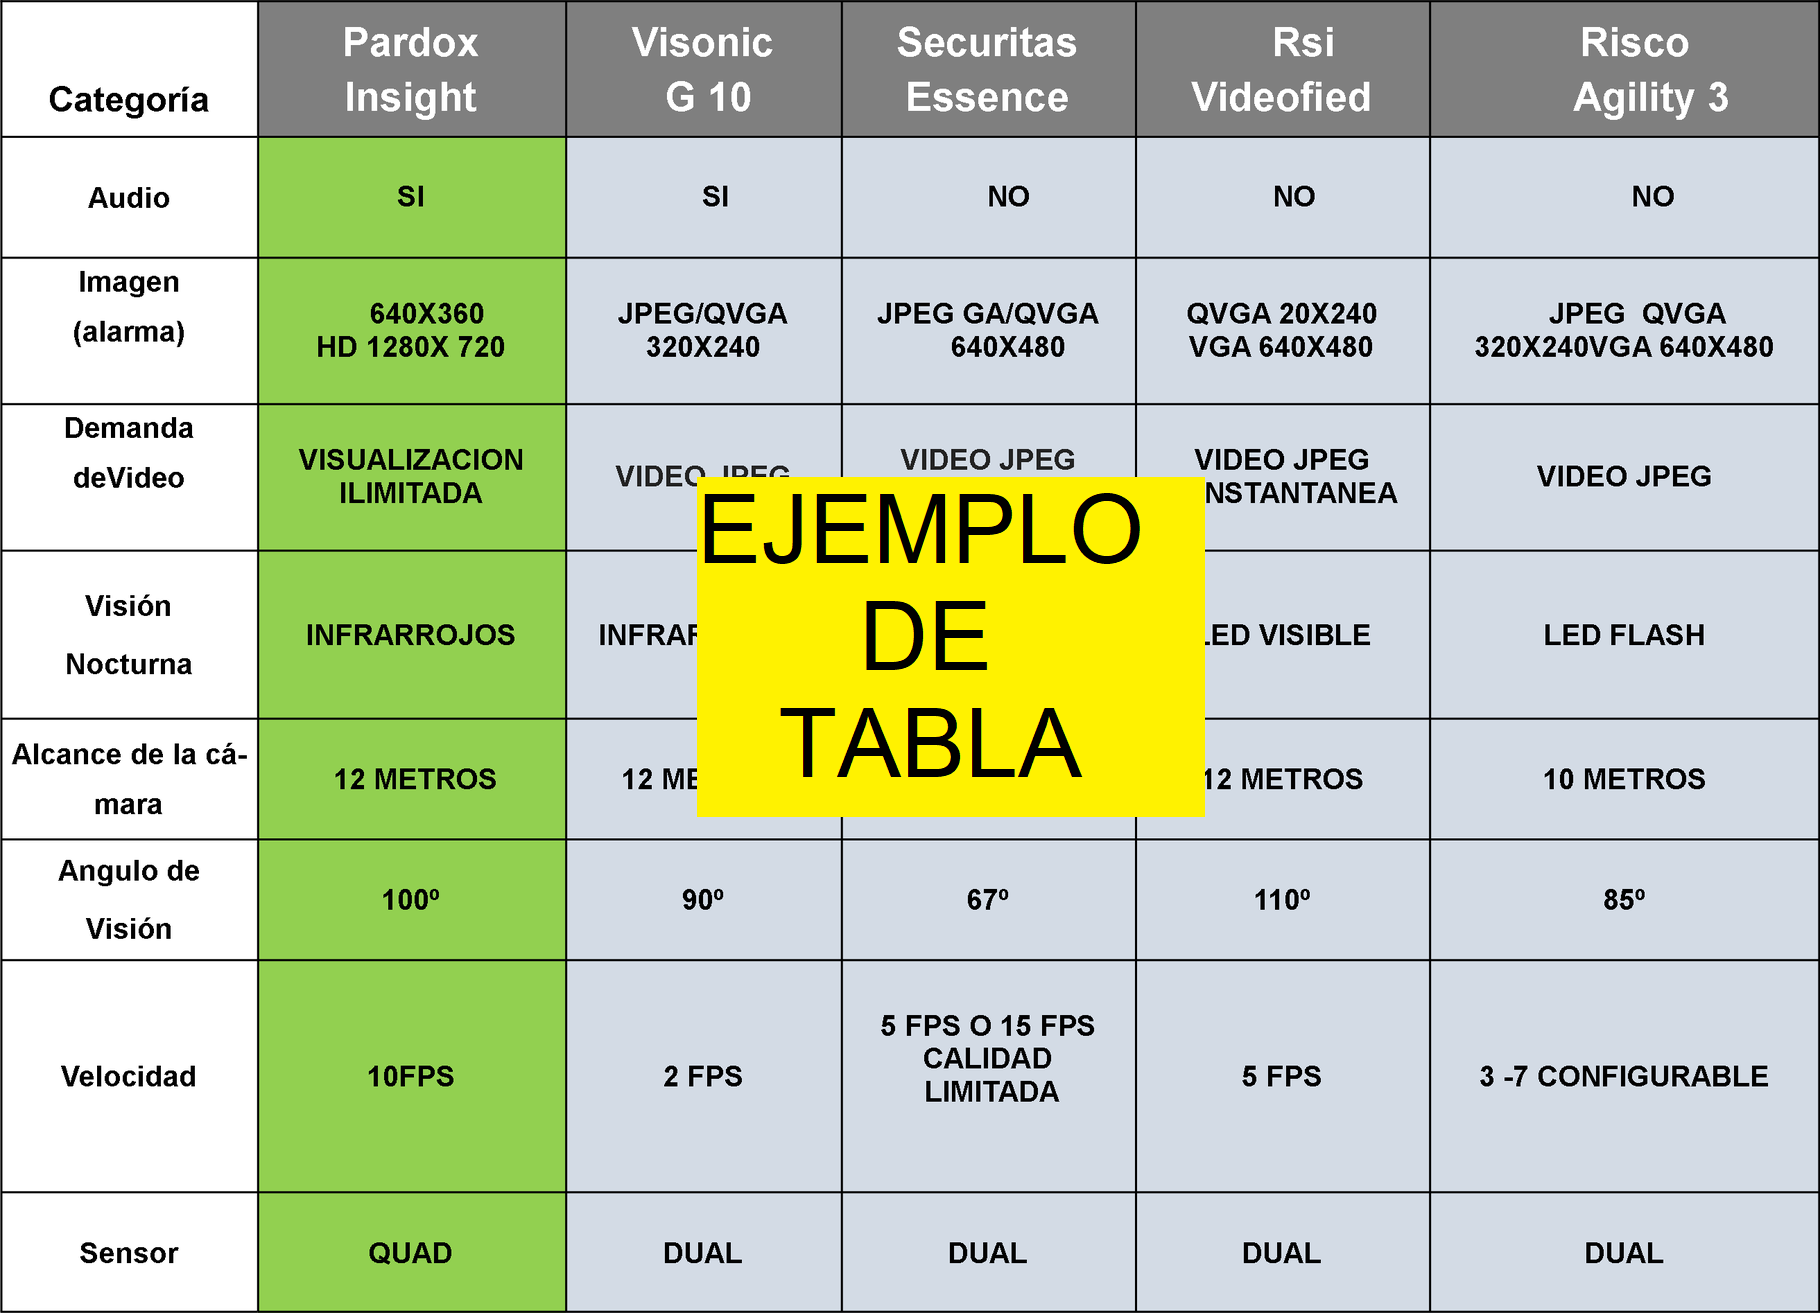
\includegraphics[width=0.85\textwidth]{chapter5/ejemplo de tabla.png}
		\caption{Ejemplo de tabla}
		\begin{myflushleftportland}
			Fuente: Elaboración propia.
		\end{myflushleftportland}
		\label{fig:ejemplo de tabla}
	\end{myfigure}
	
	Dolor sed viverra ipsum nunc aliquet bibendum. Euismod in pellentesque massa placerat. Et malesuada fames ac turpis egestas sed tempus urna. Euismod elementum nisi quis eleifend quam adipiscing vitae proin.
	
	\item \textbf{Cámara simple}
\end{itemize}



%% NUEVO SUBSECCION X.X.X.X
\subsubsection{Selección de iluminación adecuada} 


Dolor sed viverra ipsum nunc aliquet bibendum. Euismod in pellentesque massa placerat. Et malesuada fames ac turpis egestas sed tempus urna. Euismod elementum nisi quis eleifend quam adipiscing vitae proin.

%% NUEVO SUBSECCION X.X.X.X
\subsubsection{Selección de led de alta potencia}

El propósito de los leds de alta potencia es iluminar la zona en la que se realiza la captura de imágenes para detectar truchas y procesarlas. El uso de una led adecuado puede mejorar el rendimiento de la cámara. En la Figura \ref{fig:iluminacion opciones} se muestra las opciones de iluminación que se consideraron, resultando el uso de dos tiras de leds adecuadas para el sistema.

% EN LA CARPETA IMAGENES ESTAN TODA LAS IMAGENES BASE
\begin{myfigure}[H]
	\centering
	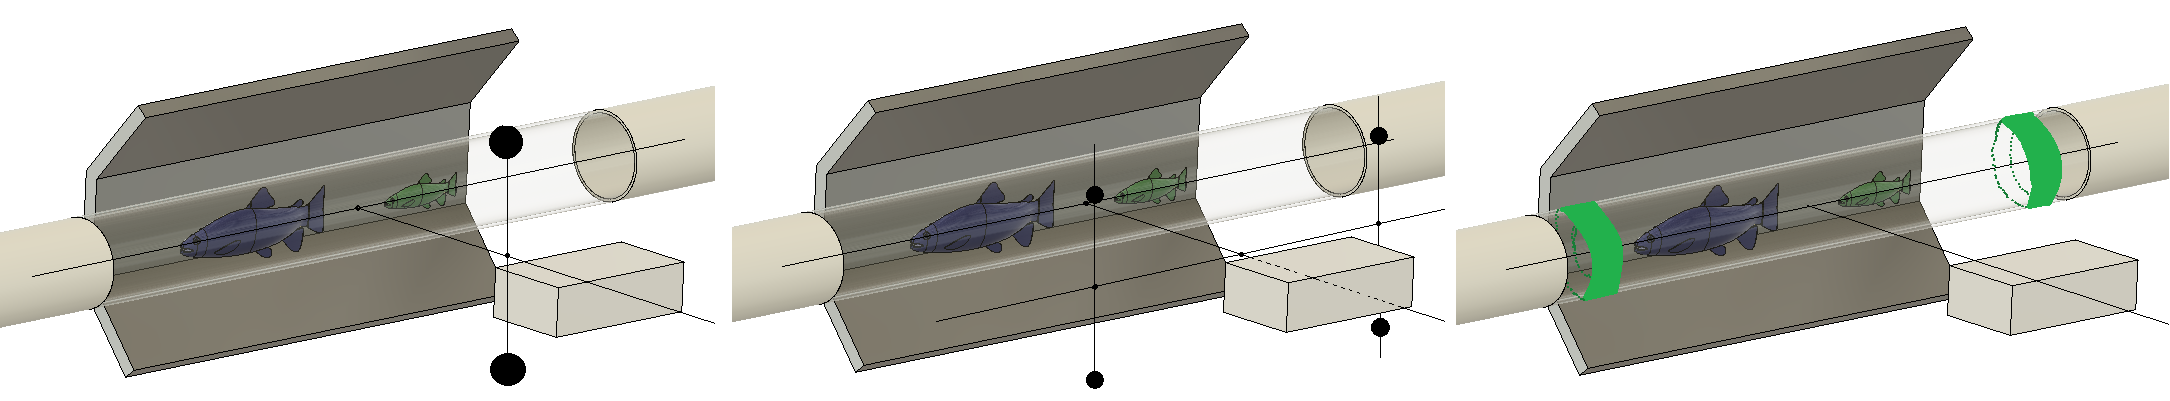
\includegraphics[width=1\textwidth]{chapter5/iluminacion opciones.png}
	\caption[Opciones de posicionamiento de iluminación.]{(Izq.) Iluminación con dos leds frente al sistema. (Cen.) Iluminación con cuatro leds frente al sistema. (Der.) Iluminación con dos tiras leds.}
	\begin{myflushleftportland}
		Fuente: Elaboración propia.
	\end{myflushleftportland}
	\label{fig:iluminacion opciones}
\end{myfigure}


La selección de una iluminación adecuada es tan importante como la selección de los otros componentes del subsistema: la ausencia de una iluminación adecuada puede degradar el rendimiento de los algoritmos, así como los de obtención de fotografías en la cámara estéreo debido al tiempo de exposición necesario por fotografía.

\begin{myequation}\label{eq:calculo de led de alta potencia}
	\begin{split}
		Iluminación_{necesaria}&=1000 %(lumenes)
	\end{split}		
\end{myequation}

En la Tabla XX se muestra una tabla técnica comparativa.

\begin{myfigure}[H]
	\centering
	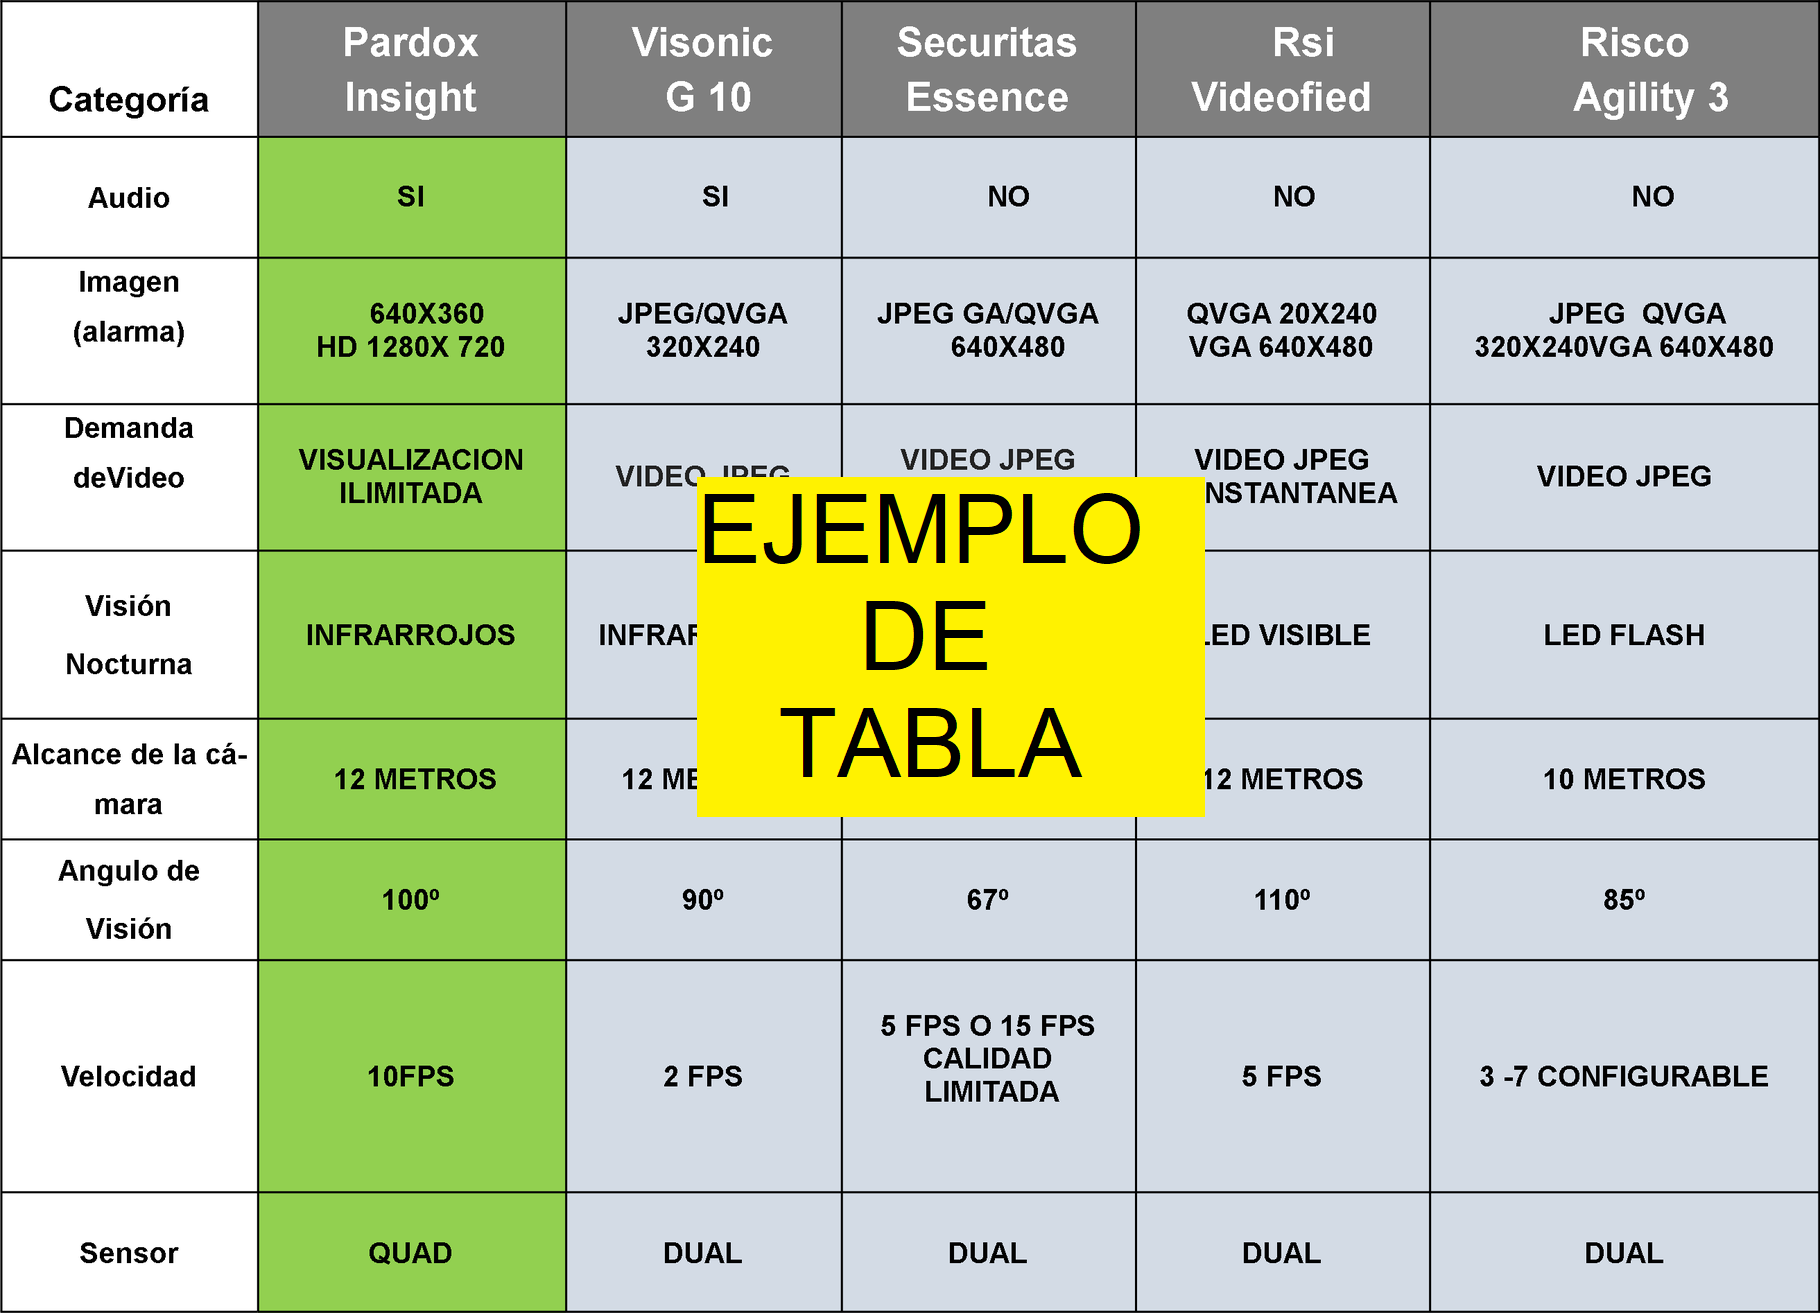
\includegraphics[width=0.85\textwidth]{chapter5/ejemplo de tabla.png}
	\caption{Ejemplo de tabla}
	\begin{myflushleftportland}
		Fuente: Elaboración propia.
	\end{myflushleftportland}
	\label{fig:ejemplo de tabla}
\end{myfigure}

%% NUEVO SUBSECCION X.X.X.X
\subsubsection{Selección de algoritmos}
\label{sssec:seleccion de algoritmos}

Los algoritmos tienen como objetivo contar y clasificar truchas. Dichos algoritmos son evaluados en la Tabla XXX mediante una comparación técnica en cuanto a diversos puntos: tiempo de respuesta, costo de hardware requerido, consumo eléctrico del hardware, ......

- NN: YOLO,YOLOv2,YOLOv3,YOLOv4,YOLOv5 \\
- NN: CNN - Fish segmentation \\
- Segmentación por características \\

Referencia a todas las versiones de YOLO. YOLO \cite{Redmon2016}, YOLO v2.0 \cite{Redmon2017}, YOLO v3.0 \cite{Redmon2018}, YOLO v4.0 \cite{Solawetz2020}, YOLO v5.0 \cite{bochkovskiy2020yolov4}.


\begin{itemize}
	
	\item \textbf{Selección de algoritmo contador de truchas} 
	
	Lorem ipsum dolor sit amet, consectetur adipiscing elit, sed do eiusmod tempor incididunt ut labore et dolore magna aliqua. Lacus sed turpis tincidunt id aliquet. Nunc aliquet bibendum enim facilisis gravida neque convallis a. Ut tellus elementum sagittis vitae et leo duis ut diam. Dolor sit amet consectetur adipiscing elit ut aliquam purus sit.
	
	\begin{myfigure}[H]
		\centering
		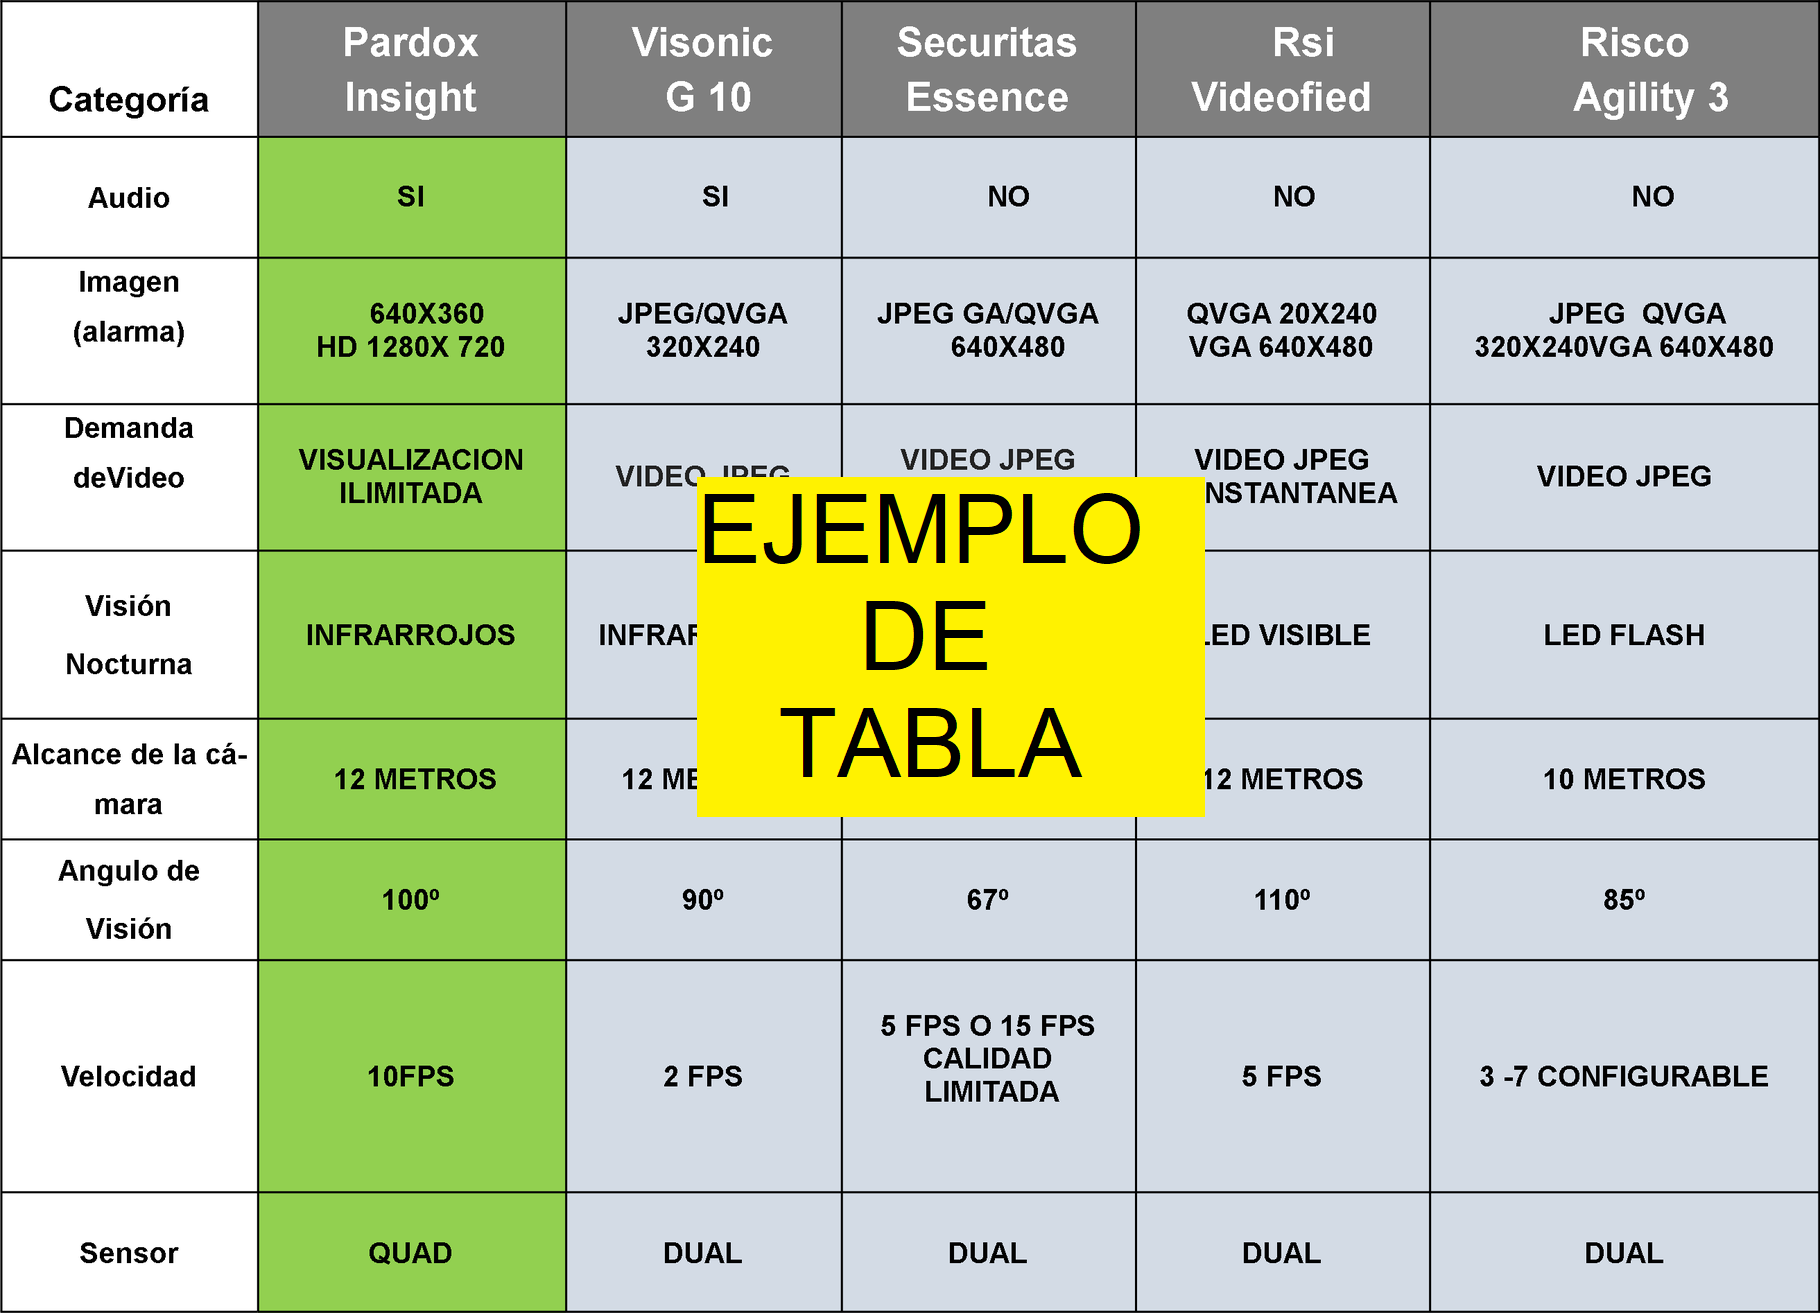
\includegraphics[width=0.85\textwidth]{chapter5/ejemplo de tabla.png}
		\caption{Ejemplo de tabla}
		\begin{myflushleftportland}
			Fuente: Elaboración propia.
		\end{myflushleftportland}
		\label{fig:ejemplo de tabla}
	\end{myfigure}

	Nunc aliquet bibendum enim facilisis gravida neque convallis a. Ut tellus elementum sagittis vitae et leo duis ut diam. Dolor sit amet consectetur adipiscing elit ut aliquam purus sit.
	
	\item \textbf{Selección de algoritmo clasificador de truchas} 
	
	Lorem ipsum dolor sit amet, consectetur adipiscing elit, sed do eiusmod tempor incididunt ut labore et dolore magna aliqua. Lacus sed turpis tincidunt id aliquet. Nunc aliquet bibendum enim facilisis gravida neque convallis a. Ut tellus elementum sagittis vitae et leo duis ut diam. Dolor sit amet consectetur adipiscing elit ut aliquam purus sit.
	
	\begin{myfigure}[H]
		\centering
		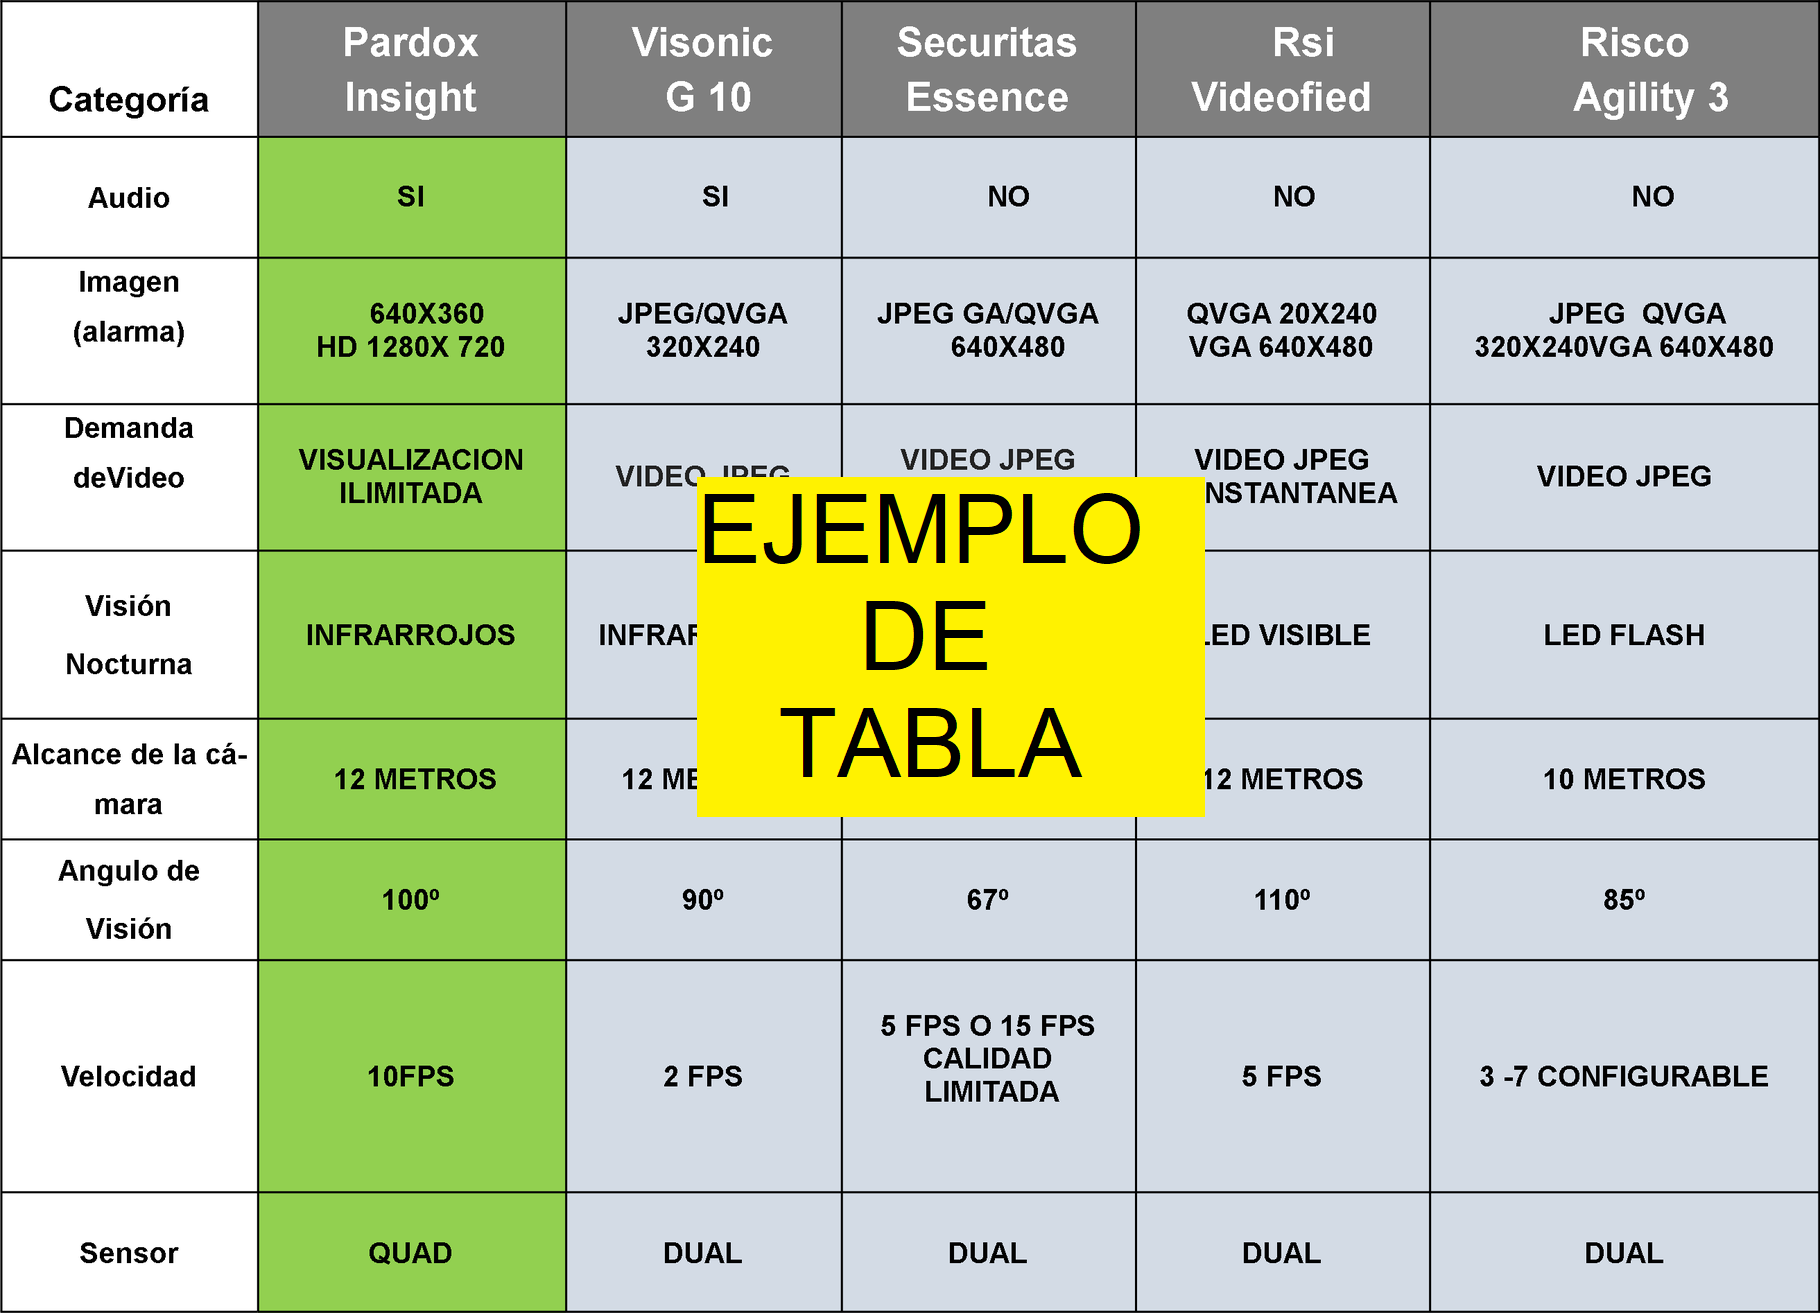
\includegraphics[width=0.85\textwidth]{chapter5/ejemplo de tabla.png}
		\caption{Ejemplo de tabla}
		\begin{myflushleftportland}
			Fuente: Elaboración propia.
		\end{myflushleftportland}
		\label{fig:ejemplo de tabla}
	\end{myfigure}
	
	Nunc aliquet bibendum enim facilisis gravida neque convallis a. Ut tellus elementum sagittis vitae et leo duis ut diam. Dolor sit amet consectetur adipiscing elit ut aliquam purus sit.
	
\end{itemize}

%% NUEVA SECCIÓN X.X.X
\subsection{Subsistema de suministro de energía}
\label{ssec:subsistema de suministro de energia}

El sistema debe suministrar energía a los diversos mecanismos electrónicos, sistemas de control y actuadores necesarios para que la máquina funcione de manera apropiada. Este subsistema debe cumplir diversos requerimientos: estar herméticamente aislado a la entrada de agua, ........\\
En los siguientes párrafos se analizaran a detalle: la selección de la batería, la selección de la fuente de alimentación, la selección de transformadores, la selección de fuentes switching, el diagrama esquemático y el diagrama eléctrico.



%% NUEVO SUBSECCION X.X.X.X
\subsubsection{Selección de la batería} 

Ut tellus elementum sagittis vitae et leo duis ut diam. Dolor sit amet consectetur adipiscing elit ut aliquam purus sit.  Dolor sit amet consectetur adipiscing elit ut aliquam purus sit. las elementum sagittis vitae et.


%% NUEVO SUBSECCION X.X.X.X
\subsubsection{Selección de fuente de alimentación} 

Lorem ipsum dolor sit amet, consectetur adipiscing elit, sed do eiusmod tempor incididunt ut labore et dolore magna aliqua. Lacus sed turpis tincidunt id aliquet. Nunc aliquet bibendum enim facilisis gravida neque convallis a. Ut tellus elementum sagittis vitae et leo duis ut diam. Dolor sit amet consectetur adipiscing elit ut aliquam purus sit. Dolor sed viverra ipsum nunc aliquet bibendum. Euismod in pellentesque massa placerat. Et malesuada fames ac turpis egestas sed tempus urna. Euismod elementum nisi quis eleifend quam adipiscing vitae proin. Ornare suspendisse sed nisi lacus sed. Mollis aliquam ut porttitor leo a diam. Varius morbi enim nunc faucibus. Sit amet purus gravida quis blandit turpis cursus in hac.

%% NUEVO SUBSECCION X.X.X.X
\subsubsection{Selección de transformadores rectificadores}

Lorem ipsum dolor sit amet, consectetur adipiscing elit, sed do eiusmod tempor incididunt ut labore et dolore magna aliqua. Lacus sed turpis tincidunt id aliquet. Nunc aliquet bibendum enim facilisis gravida neque convallis a. Ut tellus elementum sagittis vitae et leo duis ut diam. Dolor sit amet consectetur adipiscing elit ut aliquam purus sit. Dolor sed viverra ipsum nunc aliquet bibendum. Euismod in pellentesque massa placerat. Et malesuada fames ac turpis egestas sed tempus urna. Euismod elementum nisi quis eleifend quam adipiscing vitae proin. Ornare suspendisse sed nisi lacus sed. Mollis aliquam ut porttitor leo a diam. Varius morbi enim nunc faucibus. Sit amet purus gravida quis blandit turpis cursus in hac.

%% NUEVO SUBSECCION X.X.X.X
\subsubsection{Selección de fuentes switching}

Lorem ipsum dolor sit amet, consectetur adipiscing elit, sed do eiusmod tempor incididunt ut labore et dolore magna aliqua. Lacus sed turpis tincidunt id aliquet. Nunc aliquet bibendum enim facilisis gravida neque convallis a. Ut tellus elementum sagittis vitae et leo duis ut diam. Dolor sit amet consectetur adipiscing elit ut aliquam purus sit. Dolor sed viverra ipsum nunc aliquet bibendum. Euismod in pellentesque massa placerat. Et malesuada fames ac turpis egestas sed tempus urna. Euismod elementum nisi quis eleifend quam adipiscing vitae proin. Ornare suspendisse sed nisi lacus sed. Mollis aliquam ut porttitor leo a diam. Varius morbi enim nunc faucibus. Sit amet purus gravida quis blandit turpis cursus in hac.


%% NUEVO SUBSECCION X.X.X.X
\subsubsection{Diagrama esquemático} 

Ut tellus elementum sagittis vitae et leo duis ut diam. Dolor sit amet consectetur adipiscing elit ut aliquam purus sit.


%% NUEVO SUBSECCION X.X.X.X
\subsubsection{Diagrama eléctrico} 

Ut tellus elementum sagittis vitae et leo duis ut diam. Dolor sit amet consectetur adipiscing elit ut aliquam purus sit.

%% NUEVA SECCIÓN X.X.X
\subsection{Subsistema de control e interacción con el usuario}
\label{ssec:subsistema de control e interaccion con el usuario}

Nunc aliquet bibendum enim facilisis gravida neque convallis a. Ut tellus elementum sagittis vitae et leo duis ut diam. . Nunc aliquet bibendum enim facilisis gravida neque convallis a. Ut tellus elementum sagittis vitae et leo duis ut diam. 


%% NUEVO SUBSECCION X.X.X.X
\subsubsection{Selección de microcontrolador}
\label{sssec:seleccion de microcontrolador}

- Necesitamos: 80 fps \\
- Tamaño máximo: 15 cm \\
- Tamaño mínimo: 20 cm \\
- Velocidad estándar: 2 - 3 L/s (Longitud/segundos) \\
- Velocidad máxima: 3 - 4 L/s (Longitud/segundos) \\
- Debe poder: \\
---- procesar imágenes de forma rápida. \\
----  

En caso de usar NN \\
- 2 x Jetson Nano + Gumstix Jetson Nano Snapshot Board \\
- 1 x ESP32 \\

En caso de no usar NN \\
- ESP32 o Raspberry Pi 4B \\
- 1 x Jetson Nano \\

En la Sección \ref{sssec:algoritmos de deteccion de truchas}  se analiza los posibles algoritmos que pueden ser aplicados para la detección de truchas mediante visión por computadora.

Otros:\\
- Intel NSC2 \\

\begin{myfigure}[H]
	\centering
	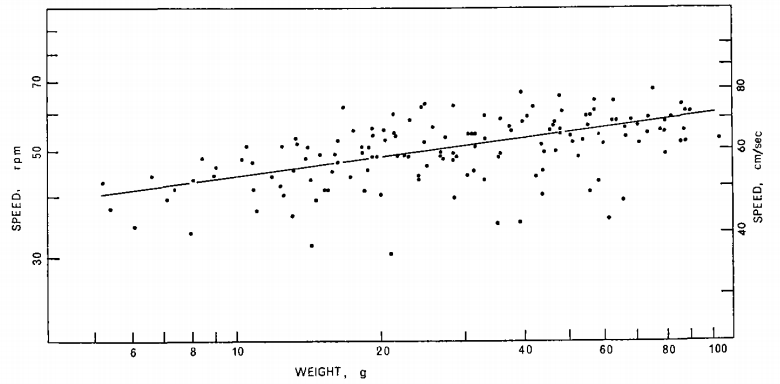
\includegraphics[width=1\textwidth]{chapter5/grafica tamano y velocidad de nado trucha arcoiris.png}
	\caption{Aproximación lineal de la relación entre peso y la velocidad de nado de truchas arcoíris}
	\begin{myflushleftportland}
		Fuente: \cite{Fry1970}
	\end{myflushleftportland}
	\label{fig:grafica tamano y velocidad de nado trucha arcoiris}
\end{myfigure}


En la Ecuación \ref{eq:ecuacion relacion tamano y velocidad de nado de trucha arcoiris} se muestra la relación entre \textit{X: peso de la trucha ($g$)} e \textit{Y: velocidad de nado ($cm/s$)} con un error \textit{Z= $\pm 0.033$}. 

\begin{myequation} \label{eq:ecuacion relacion tamano y velocidad de nado de trucha arcoiris}
	Y=-3.965+2.908(Z)X
\end{myequation}

En el caso de este trabajo, la dimensión máxima y mínima de las truchas arcoíris son de 20 cm y 15 cm, respectivamente. De la Tabla \ref{tbl:clasificacion de truchas por etapas de produccion} podemos obtener los gramos mediante interpolación lineal para cada límite: valores mínimo-máximo son 153 y 199 \textit{$g$}, respectivamente. Utilizando los valores antes indicados y empleando la Ecuación \ref{eq:ecuacion relacion tamano y velocidad de nado de trucha arcoiris} obtenemos los valores límites dentro del rango $[10.71; 15.13] (cm/s)$. Luego de escoger la máxima velocidad con redondeo hacia arriba (16 $cm/s$), ...


%% NUEVO SUBSECCION X.X.X.X
\subsubsection{Selección de indicadores}

Los indicadores ya sean visuales o sonoros son parte fundamental de una máquina. En el caso de la CCT\footnote{Máquina Contadora y Clasificadora de Truchas.} el sistema debe indicar al operario diversos estados o funciones: al detectar una trucha, al contar una trucha, al encender y al apagar.

\begin{itemize}
	\item \textbf{Indicador visual:} Lorem ipsum dolor sit amet, consectetur adipiscing elit, sed do eiusmod tempor incididunt ut labore et dolore magna aliqua. Lacus sed turpis tincidunt id aliquet. Vitae et leo duis ut diam. Dolor sit amet consectetur adipiscing elit ut aliquam purus sit. Dolor sed viverra ipsum nunc aliquet bibendum.
	
	\item \textbf{Indicador sonoro:} Una bocina indica al operario . En la Tabla \ref{tab:tabla comparativa de bocinas} se compara características técnicas entre algunas bocinas candidatas para el sistema.
	
	\begin{mytable}[H]
		\centering
		\caption{Tabla comparativa de bocinas}
		\label{tab:tabla comparativa de bocinas}
		\begin{tabular}{l|c|c|c|c|}
			\cline{2-5}
			\multicolumn{1}{c|}{\textbf{}}                         & \textbf{\begin{tabular}[c]{@{}c@{}}Requisitos\\ mínimos\end{tabular}} & \textbf{SE-B40} & \textbf{KH} & \textbf{TS-G1010F} \\ \hline
			\multicolumn{1}{|l|}{\textbf{Figura}}&
			-
			&
			\begin{minipage}{\mythirdmaxsizeofcontenttable}
				\centering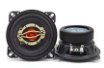
\includegraphics[width=\mythirdmaxsizeimageinsidetable]{chapter5/tablas comparativas/bocina 1.png} \\ 
				%\begin{myflushcenter}
				%	{\footnotesize Nombre imagen}
				%\end{myflushcenter}
			\end{minipage}  
			&
			\begin{minipage}{\mythirdmaxsizeofcontenttable}
				\centering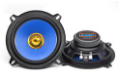
\includegraphics[width=\mythirdmaxsizeimageinsidetable]{chapter5/tablas comparativas/bocina 2.png} \\ 
				%\begin{myflushcenter}
				%	{\footnotesize Nombre imagen}
				%\end{myflushcenter}
			\end{minipage}
			&  
			\begin{minipage}{\mythirdmaxsizeofcontenttable}
				\centering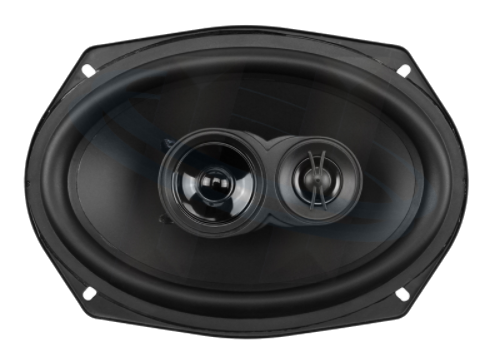
\includegraphics[width=\mythirdmaxsizeimageinsidetable]{chapter5/tablas comparativas/bocina 3.png} \\ 
				%\begin{myflushcenter}
				%	{\footnotesize Nombre imagen}
				%\end{myflushcenter}
			\end{minipage}  \\ \hline
			\multicolumn{1}{|l|}{\textbf{Fabricante}}              & -                                                                     &                 &             &                    \\ \hline
			\multicolumn{1}{|l|}{\textbf{Dimensión (cm.)}}         & -                                                                     &                 &             &                    \\ \hline
			\multicolumn{1}{|l|}{				
				\begin{minipage}{\myforthmaxsizeofcontenttable}	
					\textbf{Frecuencia de trabajo (Hz)}
				\end{minipage}
			}   & -                                                                     &                 &             &                    \\ \hline
			\multicolumn{1}{|l|}{
				\begin{minipage}{\myforthmaxsizeofcontenttable}	
					\textbf{Voltaje de alimentación (V)}
				\end{minipage}
			} & -                                                                     & 12 VDC          & 12 VDC      & 12 VDC             \\ \hline
			\multicolumn{1}{|l|}{\textbf{RMS (W)}}                 & -                                                                     & 80              & 25          & 30                 \\ \hline
			\multicolumn{1}{|l|}{\textbf{Precio (S/)}}             & -                                                                     & 105             & 105         & 79                 \\ \hline
			\multicolumn{1}{|l|}{\textbf{Disponibilidad}}          & Inmediata                                                             & A pedido        & A pedido    & A pedido           \\ \hline
		\end{tabular}
		\begin{flushleft}	
			Fuente: Imágenes de dominio público y elaboración propia.
		\end{flushleft}
	\end{mytable}
	
\end{itemize}



%% NUEVO SUBSECCION X.X.X.X
\subsubsection{Selección de interruptor de seguridad de apagado de emergencia}

La implementación de un interruptor de seguridad es muy importante en el diseño de máquinas ya que es el mecanismo físico por el cual podemos parar la máquina quitando el suministro eléctrico a todos los componentes. En la Tabla \ref{tab:tabla comparativa de interruptor de seguridad de apagado de emergencia} se compara características técnicas entre interruptor de seguridad candidatos para el sistema.

\begin{mytable}[H]
	\centering
	\caption{Tabla comparativa de interruptor de seguridad de apagado de emergencia.}
	\label{tab:tabla comparativa de interruptor de seguridad de apagado de emergencia}
	\begin{tabular}{l|c|c|c|c|}
		\cline{2-5}
		\multicolumn{1}{c|}{\textbf{}}                          & \textbf{\begin{tabular}[c]{@{}c@{}}Requisitos\\ mínimos\end{tabular}} & \textbf{1} & \textbf{2} & \textbf{3} \\ \hline
		\multicolumn{1}{|l|}{\textbf{Figura}}&
		-
		&
		\begin{minipage}{\mythirdmaxsizeofcontenttable}
			\centering
\includegraphics[width=\mythirdmaxsizeimageinsidetable]{chapter5/tablas comparativas/interruptor de seguridad de apagado de emergencia 1.png} \\ 
			%\begin{myflushcenter}
			%	{\footnotesize Nombre imagen}
			%\end{myflushcenter}
		\end{minipage}  
		&
		\begin{minipage}{\mythirdmaxsizeofcontenttable}
			\centering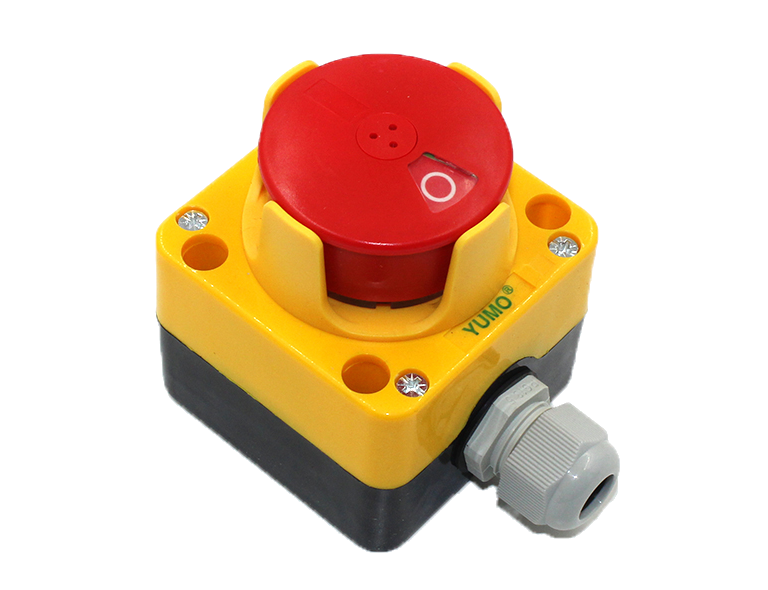
\includegraphics[width=\mythirdmaxsizeimageinsidetable]{chapter5/tablas comparativas/interruptor de seguridad de apagado de emergencia 2.png} \\ 
			%\begin{myflushcenter}
			%	{\footnotesize Nombre imagen}
			%\end{myflushcenter}
		\end{minipage}
		&  
		\begin{minipage}{\mythirdmaxsizeofcontenttable}
			\centering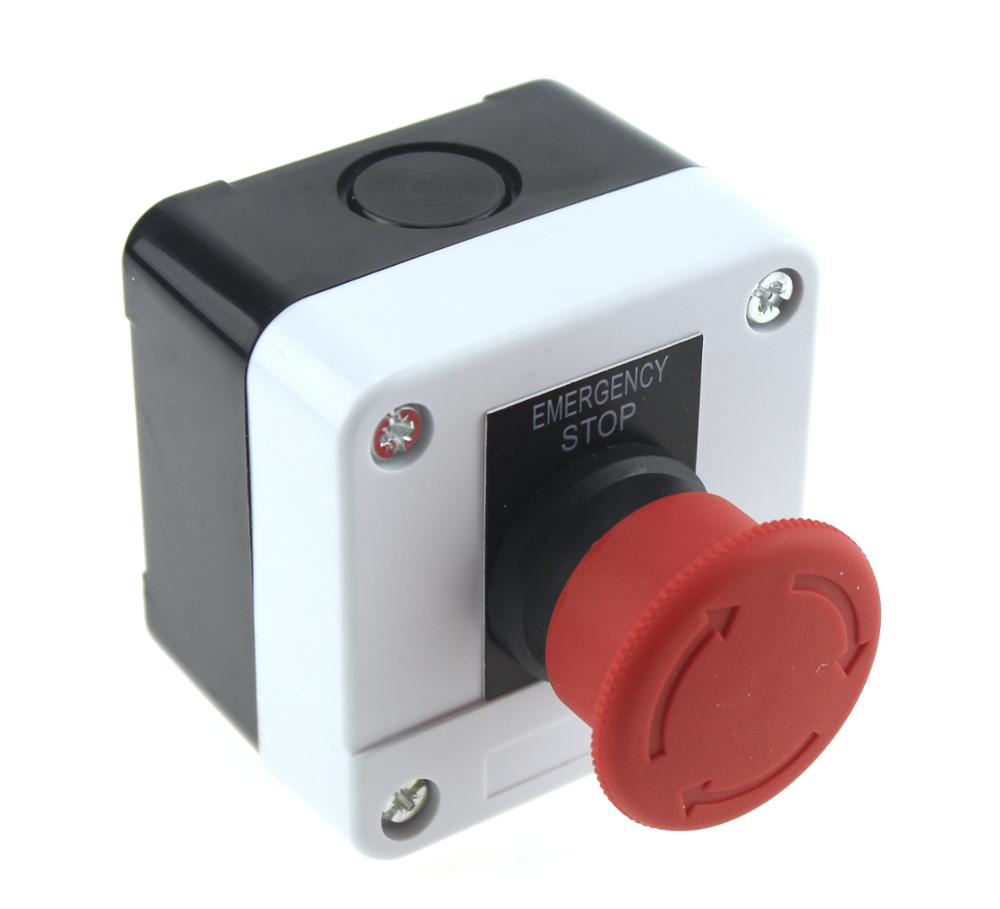
\includegraphics[width=\mythirdmaxsizeimageinsidetable]{chapter5/tablas comparativas/interruptor de seguridad de apagado de emergencia 3.png} \\ 
			%\begin{myflushcenter}
			%	{\footnotesize Nombre imagen}
			%\end{myflushcenter}
		\end{minipage}  \\ \hline
		\multicolumn{1}{|l|}{\textbf{Fabricante}}               & -                                                                     & 9          & 10         & 11         \\ \hline
		\multicolumn{1}{|l|}{\textbf{Nivel de protección}}      & 12                                                                    & 13         & 14         & 15         \\ \hline
		\multicolumn{1}{|l|}{
			\begin{minipage}{\myforthmaxsizeofcontenttable}			
				\textbf{Máximo voltaje admisible (V)}
			\end{minipage}
		}
		&
		16
		& 17         & 18         & 19         \\ \hline
		\multicolumn{1}{|l|}{
			\begin{minipage}{\myforthmaxsizeofcontenttable}			
				\textbf{Diámetro del botón (mm.)}
			\end{minipage}
		} & 20                                                                    & 21         & 22         & 23         \\ \hline
		\multicolumn{1}{|l|}{\textbf{Precio (S/)}}              & 24                                                                    & 25         & 26         & 27         \\ \hline
		\multicolumn{1}{|l|}{\textbf{Disponibilidad}}           & 32                                                                    & 33         & 34         & 35         \\ \hline
	\end{tabular}
	\begin{flushleft}	
		Fuente: Imágenes de dominio público y elaboración propia.
	\end{flushleft}
\end{mytable}


%% NUEVO SUBSECCION X.X.X.X
\subsubsection{Selección de interruptor de interruptor tipo hongo}

El encendido o apagado de la máquina es realizado por este interruptor, es decir, el control del suministro de energía del sistema depende de dicho dispositivo. En la Tabla \ref{tab:tabla comparativa de interruptor de interruptor tipo hongo} se compara características técnicas entre interruptores tipo hongo candidatos para el sistema.

\begin{mytable}[H]
\centering
\caption{Tabla comparativa de interruptor de interruptor tipo hongo.}
\label{tab:tabla comparativa de interruptor de interruptor tipo hongo}
\begin{tabular}{l|c|c|c|c|}
	\cline{2-5}
	\multicolumn{1}{c|}{\textbf{}}                          & \textbf{\begin{tabular}[c]{@{}c@{}}Requisitos\\ mínimos\end{tabular}} & \textbf{1} & \textbf{2} & \textbf{3} \\ \hline
	\multicolumn{1}{|l|}{\textbf{Figura}}&
	-
	&
	\begin{minipage}{\mythirdmaxsizeofcontenttable}
		\centering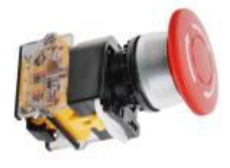
\includegraphics[width=\mythirdmaxsizeimageinsidetable]{chapter5/tablas comparativas/interruptor tipo hongo 1.png} \\ 
		%\begin{myflushcenter}
		%	{\footnotesize Nombre imagen}
		%\end{myflushcenter}
	\end{minipage}  
	&
	\begin{minipage}{\mythirdmaxsizeofcontenttable}
		\centering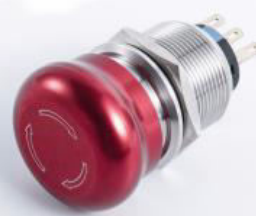
\includegraphics[width=\mythirdmaxsizeimageinsidetable]{chapter5/tablas comparativas/interruptor tipo hongo 2.png} \\ 
		%\begin{myflushcenter}
		%	{\footnotesize Nombre imagen}
		%\end{myflushcenter}
	\end{minipage}
	&  
	\begin{minipage}{\mythirdmaxsizeofcontenttable}
		\centering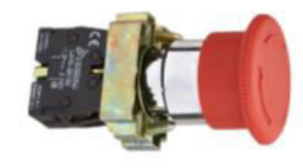
\includegraphics[width=\mythirdmaxsizeimageinsidetable]{chapter5/tablas comparativas/interruptor tipo hongo 3.png} \\ 
		%\begin{myflushcenter}
		%	{\footnotesize Nombre imagen}
		%\end{myflushcenter}
	\end{minipage}  \\ \hline
	\multicolumn{1}{|l|}{\textbf{Fabricante}}               & -                                                                     & 9          & 10         & 11         \\ \hline
	\multicolumn{1}{|l|}{\textbf{Nivel de protección}}      & 12                                                                    & 13         & 14         & 15         \\ \hline
	\multicolumn{1}{|l|}{
		\begin{minipage}{\myforthmaxsizeofcontenttable}			
			\textbf{Máximo voltaje admisible (V)}
		\end{minipage}
	}
	&
	16
	& 17         & 18         & 19         \\ \hline
	\multicolumn{1}{|l|}{
			\begin{minipage}{\myforthmaxsizeofcontenttable}			
				\textbf{Diámetro del botón (mm.)}
			\end{minipage}
	} & 20                                                                    & 21         & 22         & 23         \\ \hline
	\multicolumn{1}{|l|}{\textbf{Precio (S/)}}              & 24                                                                    & 25         & 26         & 27         \\ \hline
	\multicolumn{1}{|l|}{\textbf{Disponibilidad}}           & 32                                                                    & 33         & 34         & 35         \\ \hline
\end{tabular}
\begin{flushleft}	
	Fuente: Imágenes de dominio público y elaboración propia.
\end{flushleft}
\end{mytable}

%% NUEVO SUBSECCION X.X.X.X
\subsubsection{Cálculo del consumo de energía del sistema} 

El cálculo del consumo de energía del sistema es la suma de potencia requerida por cada componente. Dicha información se presenta en la Tabla \ref{fig:potencia requerida por componente}, además se muestra el modelo, la potencia máxima, voltaje de cada componente. Se considera, también, la cantidad de cada modelo de componente electrónico usado en el sistema.

% TIENE QUE SER TABLA
% TIENE QUE SER TABLA
% TIENE QUE SER TABLA
% TIENE QUE SER TABLA
% TIENE QUE SER TABLA
     
\begin{myfigure}[H]
	\centering
	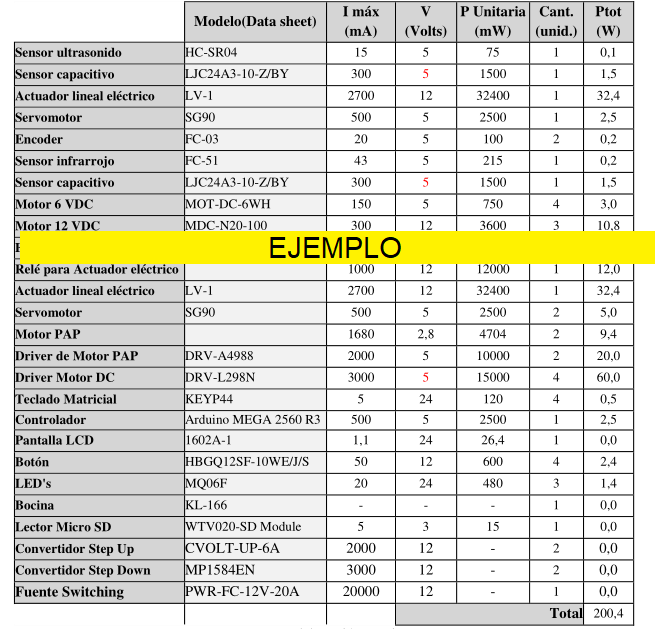
\includegraphics[width=1\textwidth]{chapter5/potencia requerida por componente.png}
	\caption{Potencia requerida por componente}
	\begin{myflushleftportland}
		Fuente: Elaboración propia.
	\end{myflushleftportland}
	\label{fig:potencia requerida por componente}
\end{myfigure}


%% NUEVO SUBSECCION X.X.X.X
\subsubsection{Diagrama de flujo}

El diagrama de flujo principal, expuesto en la Figura \ref{fig:diagrama de flujo} describe los pasos necesarios para el control del sistema. .. ... .. [Explicar diagrama de flujo]

\begin{myfigure}[H]
	\centering
	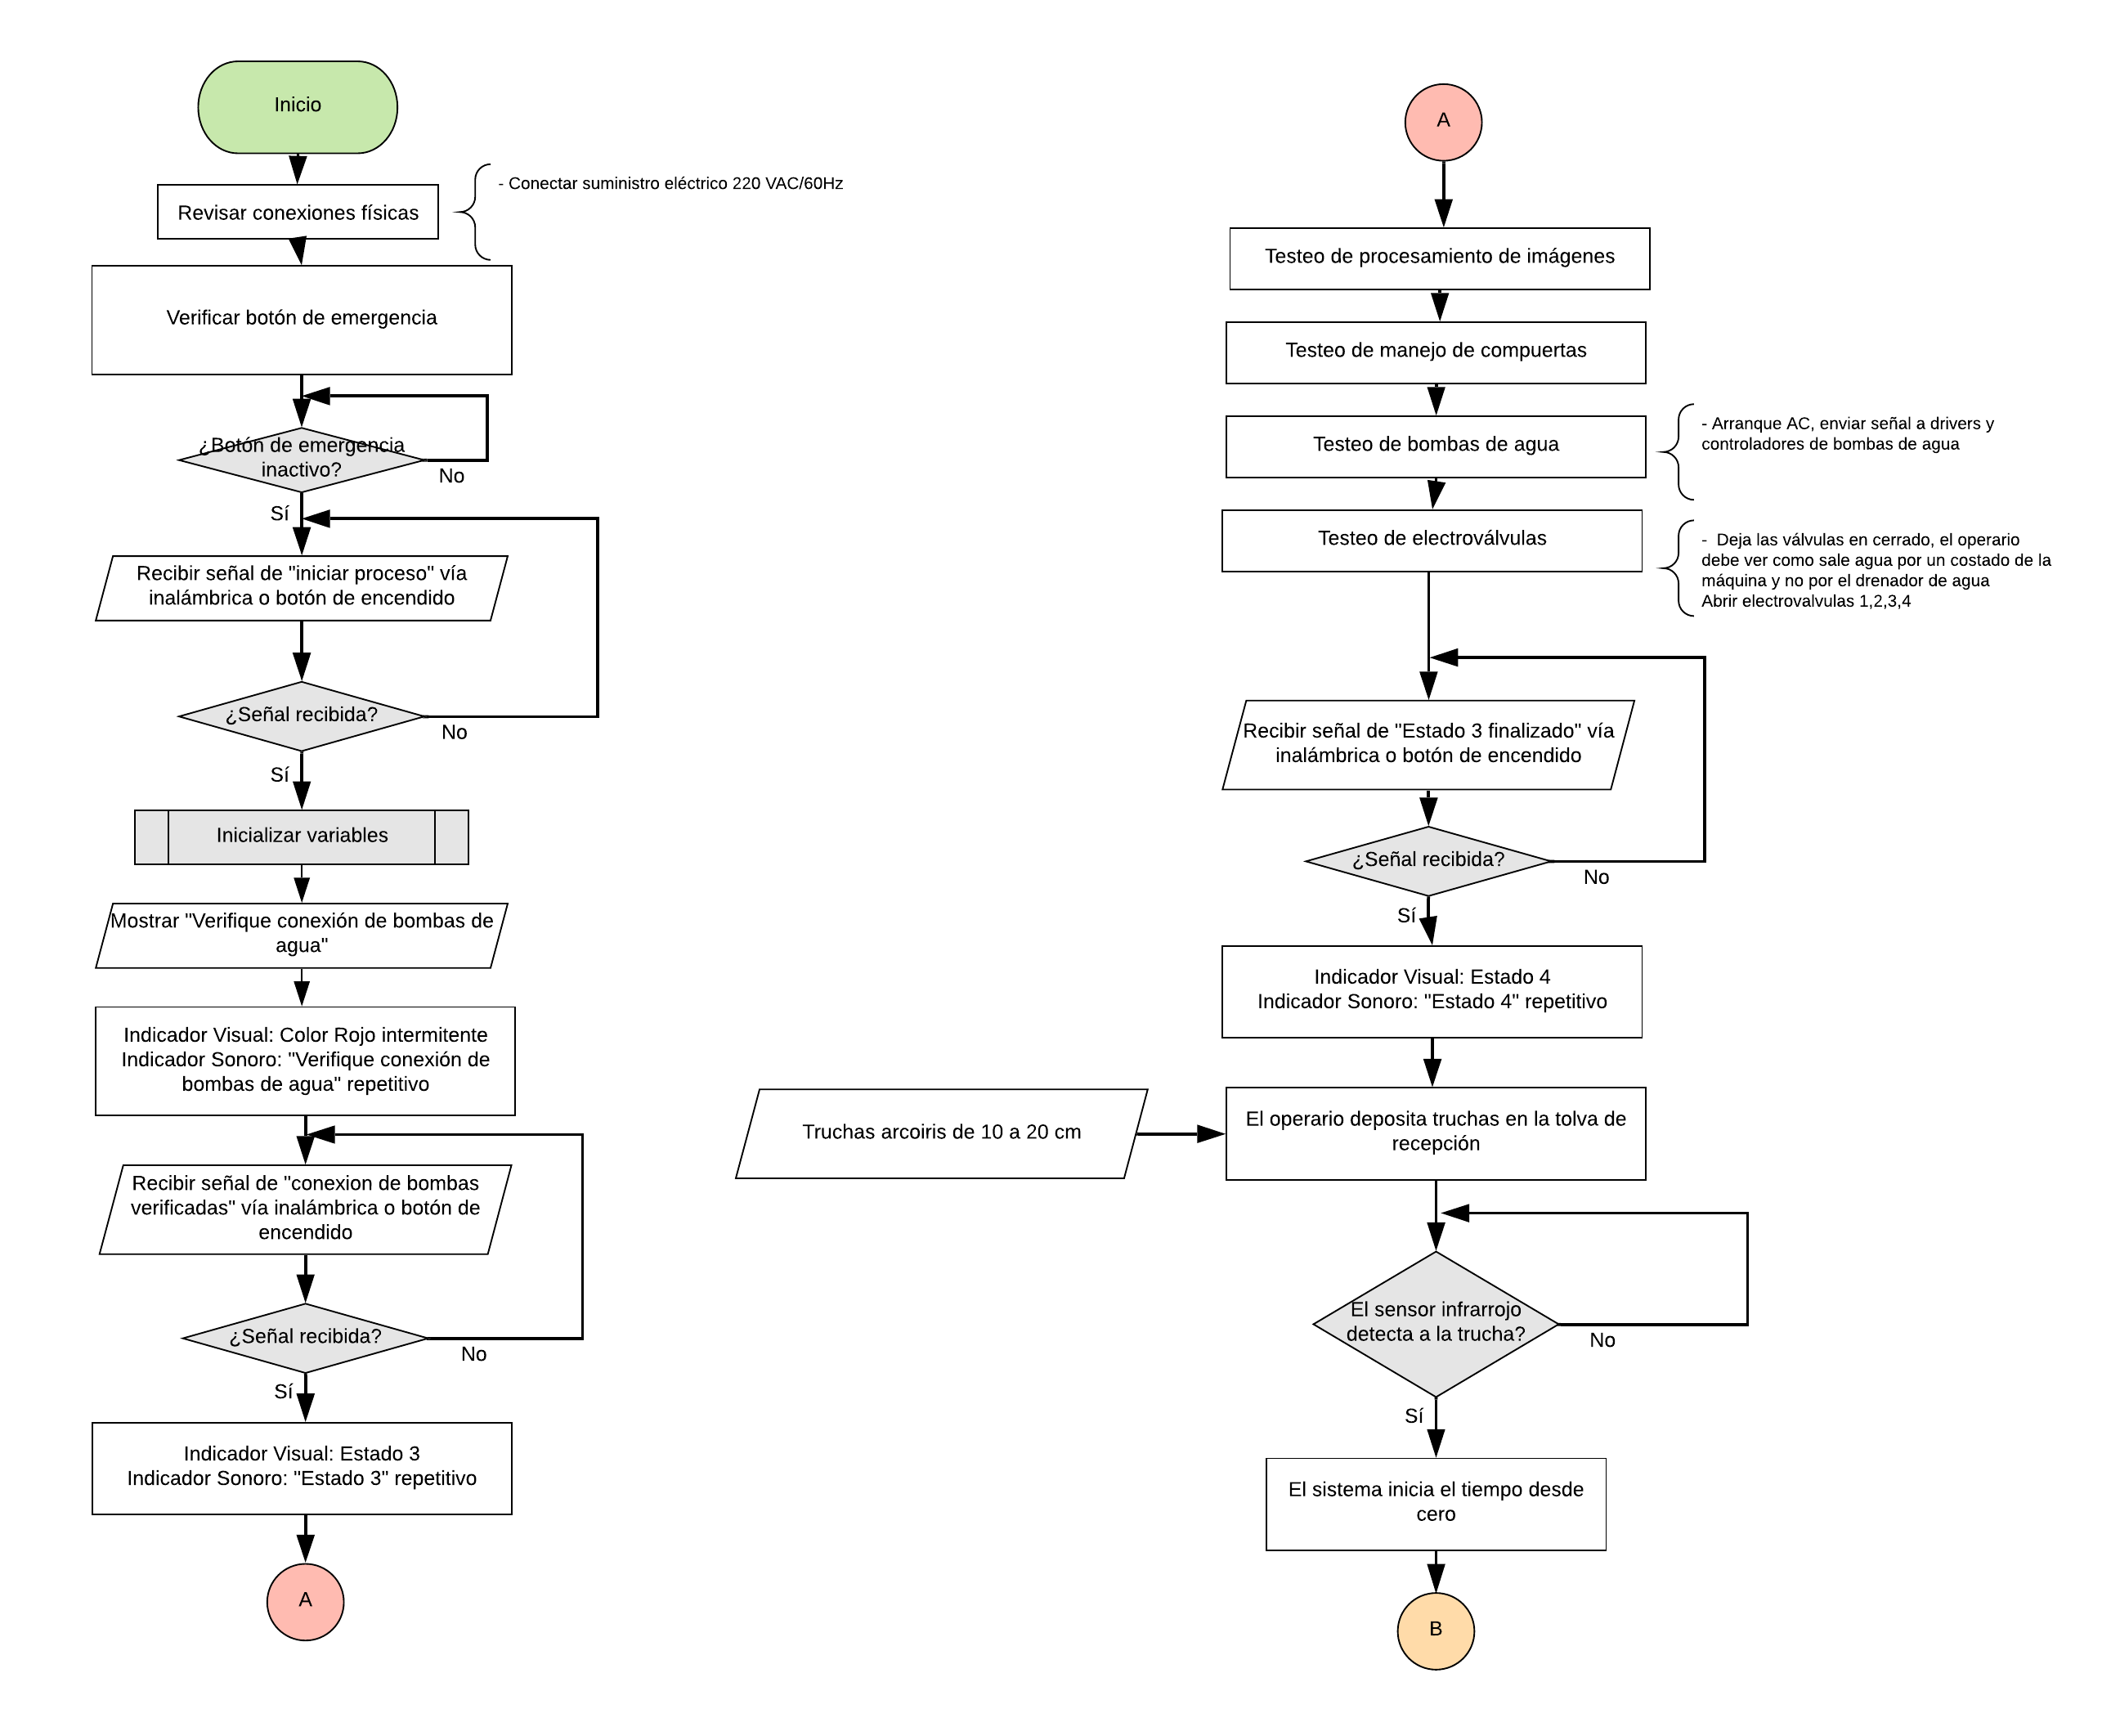
\includegraphics[width=1\textwidth]{chapter5/diagrama de flujo.png}
	\caption{Diagrama de flujo principal}
	\begin{myflushleftportland}
		Fuente: Elaboración propia.
	\end{myflushleftportland}
	\label{fig:diagrama de flujo}
\end{myfigure}


%% NUEVO SUBSECCION X.X.X.X
\subsubsection{Diseño frontend de la aplicación móvil}

La aplicación móvil permitirá a un operario visualizar los estados de la máquina, así como tener un registro de la clasificación y conteo de truchas, es decir, extraer los datos luego de ser procesados por la máquina CCT de manera inalámbrica al terminar el proceso. Además, posterior a este trabajo, podría agregarse más características al aplicativo móvil. El framework de desarrollo del aplicativo, que no se desarrollará en el presente trabajo, escogido es Flutter por su paradigma multiplataforma, es decir, escribir un programa que se vea igual en los sistemas operativos Android y iOS \cite{Simone2020}. El diseño frontend escogido para el proyecto y su desarrollo sencillo 

Designing the obvious
\cite{Joekman2010} \\
Google Flutter Mobile Development Quick Start Guide
\cite{PrajyotMainkar2019} \\
Mobile Learning Design: Theories and Application
\cite{Churchill2016} \\
Mobile Design Pattern Gallery: UI Patterns for Mobile Applications
\cite{Neil2012}


\begin{myfigure}[H]
	\centering
	
\includegraphics[width=1\textwidth]{chapter5/aplicacion movil login.png}
	\caption{Aplicación móvil: inicio de sesión}
	\begin{myflushleftportland}
		Fuente: Elaboración propia.
	\end{myflushleftportland}
	\label{fig:aplicacion movil login}
\end{myfigure}


%% NUEVA SECCIÓN X.X.X
\subsection{Subsistema de flotación}
\label{ssec:subsistema de flotacion}

Luego de definir en las Secciones \ref{ssec:subsistema de recepcion y traslado de truchas}, \ref{ssec:subsistema de procesamiento de imágenes}, \ref{ssec:subsistema de suministro de energia}, y \ref{ssec:subsistema de control e interaccion con el usuario}, la selección de los dispositivos y su interacción el sistema permiten calcular las dimensiones de la máquina para analizar la flotabilidad y seleccionar flotadores adecuados. En las siguientes subsecciones se analizan los cálculos, selección y diseño del sistema de flotación.

%% NUEVO SUBSECCION X.X.X.X
\subsubsection{Cálculo de sistema flotador}

Lacus sed turpis tincidunt id aliquet. Nunc aliquet bibendum enim facilisis gravida neque convallis a. Ut tellus elementum sagittis vitae et leo duis ut diam. Dolor sit amet consectetur adipiscing elit ut aliquam purus sit. 

%% NUEVO SUBSECCION X.X.X.X
\subsubsection{Selección de flotadores}

Lacus sed turpis tincidunt id aliquet. Nunc aliquet bibendum enim facilisis gravida neque convallis a. Ut tellus elementum sagittis vitae et leo duis ut diam. Dolor sit amet consectetur adipiscing elit ut aliquam purus sit. 


\begin{mytable}[H]
	\centering
	\caption{Tabla comparativa de flotadores.}
	\label{tab:tabla comparativa de flotadores}
	\begin{tabular}{l|c|c|c|c|}
		\cline{2-5}
		\multicolumn{1}{c|}{\textbf{}}                          & \textbf{\begin{tabular}[c]{@{}c@{}}Requisitos\\ mínimos\end{tabular}} & \textbf{1} & \textbf{2} & \textbf{3} \\ \hline
		\multicolumn{1}{|l|}{\textbf{Figura}}&
		-
		&
		\begin{minipage}{\mythirdmaxsizeofcontenttable}
			\centering
\includegraphics[width=\mythirdmaxsizeimageinsidetable]{chapter5/tablas comparativas/flotador 1.png} \\ 
			%\begin{myflushcenter}
			%	{\footnotesize Nombre imagen}
			%\end{myflushcenter}
		\end{minipage}  
		&
		\begin{minipage}{\mythirdmaxsizeofcontenttable}
			\centering
\includegraphics[width=\mythirdmaxsizeimageinsidetable]{chapter5/tablas comparativas/flotador 2.png} \\ 
			%\begin{myflushcenter}
			%	{\footnotesize Nombre imagen}
			%\end{myflushcenter}
		\end{minipage}
		&  
		\begin{minipage}{\mythirdmaxsizeofcontenttable}
			\centering
\includegraphics[width=\mythirdmaxsizeimageinsidetable]{chapter5/tablas comparativas/flotador 3.png} \\ 
			%\begin{myflushcenter}
			%	{\footnotesize Nombre imagen}
			%\end{myflushcenter}
		\end{minipage}  \\ \hline
		\multicolumn{1}{|l|}{\textbf{Fabricante}}               & -                                                                     & 9          & 10         & 11         \\ \hline
		\multicolumn{1}{|l|}{\textbf{Característica}}      & 12                                                                    & 13         & 14         & 15         \\ \hline
		\multicolumn{1}{|l|}{
			\begin{minipage}{\myforthmaxsizeofcontenttable}			
				\textbf{Característica}
			\end{minipage}
		}
		&
		16
		& 17         & 18         & 19         \\ \hline
		\multicolumn{1}{|l|}{
			\begin{minipage}{\myforthmaxsizeofcontenttable}			
				\textbf{Característica}
			\end{minipage}
		} & 20                                                                    & 21         & 22         & 23         \\ \hline
		\multicolumn{1}{|l|}{\textbf{Característica}}              & 24                                                                    & 25         & 26         & 27         \\ \hline
		\multicolumn{1}{|l|}{\textbf{Característica}}           & 32                                                                    & 33         & 34         & 35         \\ \hline
	\end{tabular}
	\begin{flushleft}	
		Fuente: Imágenes de dominio público y elaboración propia.
	\end{flushleft}
\end{mytable}

%% NUEVO SUBSECCION X.X.X.X
\subsubsection{Diseño de sistema de flotación}

Lacus sed turpis tincidunt id aliquet. Nunc aliquet bibendum enim facilisis gravida neque convallis a. Ut tellus elementum sagittis vitae et leo duis ut diam. Dolor sit amet consectetur adipiscing elit ut aliquam purus sit. 



%% NUEVA SECCIÓN X.X.X
\subsection{Planos del sistema}
\label{ssec:planos del sistema}

Los planos permiten visualizar el sistema de una forma en particular dependiendo del tipo de plano. En el presente trabajo optaremos por incluir dos tipos: planos de ensamble y planos de despiece.

%% NUEVO SUBSECCION X.X.X.X
\subsubsection{Lista de planos de ensamble}

Un plano de ensamble presenta una visión de las diferentes partes que van juntas, cada componente va listada y se proporcionan características técnicas como el  tipo de material y cantidad de componentes similares.\footnote{\cite{Goetsch2010}} En la Tabla XXX se muestra una lista de planos de ensamble.


\begin{mytable}[H]
	\centering
	\caption{Lista de planos de ensamble.}
	\label{tab:lista de planos de ensamble}
	\begin{tabular}{|c|c|c|}
		\hline
		\textbf{N° Lámina} & \textbf{Plano} & \textbf{Tipo} \\ \hline
		\textbf{L1}        & 1              & 2             \\ \hline
		\textbf{L2}        & 3              & 4             \\ \hline
		\textbf{L3}        & 5              & 6             \\ \hline
		\textbf{L4}        & 7              & 8             \\ \hline
		\textbf{L5}        & 9              & 10            \\ \hline
		\textbf{L6}        & 11             & 12            \\ \hline
		\textbf{L7}        & 13             & 14            \\ \hline
	\end{tabular}
	\begin{flushleft}	
	Fuente: Imágenes de dominio público y elaboración propia.
\end{flushleft}
\end{mytable}


%% NUEVO SUBSECCION X.X.X.X
\subsubsection{Plano de despiece}

Lacus sed turpis tincidunt id aliquet. Nunc aliquet bibendum enim facilisis gravida neque convallis a. Ut tellus elementum sagittis vitae et leo duis ut diam. Dolor sit amet consectetur adipiscing elit ut aliquam purus sit. 


\begin{myfigure}[H]
	\centering
	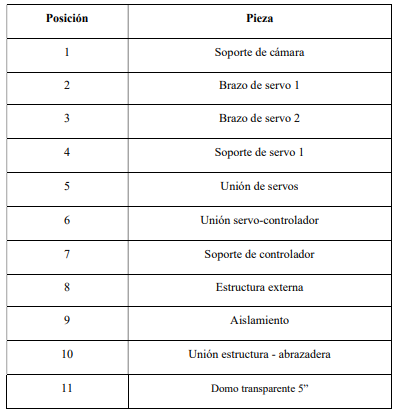
\includegraphics[width=0.5\textwidth]{chapter5/ejemplo tabla plano despiece.png}
	\caption{...}
	\begin{myflushleftportland}
		Fuente: ...
	\end{myflushleftportland}
	\label{fig:ejemplo tabla plano despiece}
\end{myfigure}